%\documentclass[11pt, a4paper, twoside]{report}
\documentclass[11pt, a4paper]{memoir}
\usepackage[T1]{fontenc}
\usepackage[latin1]{inputenc}
\usepackage{amsmath,epsfig,latexsym,bm,textcomp}
\usepackage{mathtools}
\usepackage{amssymb,amsthm}
\usepackage[a4paper, top=3cm, bottom=3cm, left=2.5cm, right=2.5cm]{geometry}
%\usepackage{fancyhdr}
\usepackage{color}
\usepackage{mathrsfs}
\usepackage{bbm}
%\usepackage{accents}
\usepackage{graphicx}
%\usepackage{enumitem}
\usepackage{needspace}

%\usepackage{kpfonts}
%\usepackage{yhmath}
%\let\wwidehat\widehat

%\usepackage[mathx,mathb,matha]{mathabx} % \widecheck
%\usepackage{accents}

\usepackage{url}

%\chapterstyle{verville}

%\usepackage{avant}
%\usepackage{bookman}
%\usepackage{helvet}
%\usepackage{newcent}
%\usepackage{palatino}
%\usepackage{times}

%\usepackage[sc]{mathpazo} \linespread{1.05} %tohle je pekne
%\usepackage{concmath} %hustota
%\usepackage{txfonts}
%\usepackage[light,math]{iwona}
%\usepackage{iwona}
%\usepackage{mathptmx}
%\usepackage{fourier}
%\usepackage[math]{anttor} %zajimave
%\usepackage[light,math]{anttor}
%\usepackage[condensed,math]{anttor}
%\usepackage{concmath} %hustota
%\usepackage{gfsartemisia} %nejde i s tremou, ale jinak pekne
%\usepackage{kmath,kerkis} % The order of the packages matters; kmath changes the default text font
%\usepackage{kerkis}
%\usepackage{fouriernc}

\makepagestyle{ruled}
\nouppercaseheads
\makeevenfoot{ruled}{}{\thepage}{}
\makeoddfoot{ruled}{}{\thepage}{}
\makeheadrule{ruled}{\textwidth}{\normalrulethickness}
%\makeevenhead{ruled}{\scshape \leftmark}{}{} % small caps
%\makeoddhead{ruled}{}{}{\scshape \rightmark}
\makeevenhead{ruled}{\textsf \leftmark}{}{} % small caps
\makeoddhead{ruled}{}{}{\textsf \rightmark}

\pagestyle{ruled}

\begin{document}

\newtheoremstyle{theo}{}{}{\slshape}{}{\bfseries}{.}{ }{}

\theoremstyle{definition}
\newtheorem{definition}{Definition}[chapter]

\theoremstyle{theo}
%\theoremstyle{plain}
\newtheorem{theorem}[definition]{Theorem}%[chapter]
\newtheorem{proposition}[definition]{Proposition}%[chapter]
\newtheorem{lemma}[definition]{Lemma}%[chapter]
\newtheorem{corollary}[definition]{Corollary}%[chapter]
\newtheorem*{fact}{Fact}

\theoremstyle{remark}
\newtheorem*{remark}{Remark}
\newtheorem*{remarks}{Remarks}
\newtheorem*{recall}{Recall}
\newtheorem*{exercise}{Exercise}
\newtheorem*{example}{Example}
\newtheorem*{examples}{Examples}
\newtheorem*{contrex}{Counterexample}
\newtheorem*{convention}{Convention}

%\def\ins{\if@display\mkern12mu\else\mkern6mu\fi\rule{7pt}{0.4pt}\rule{0.4pt}{7pt}\if@display\mkern12mu\else\mkern6mu\fi}

\def\ins{\operatorname{\without}}

%\newcommand{\indep}{\perp\!\!\!\perp}
\newcommand\indep{\protect\mathpalette{\protect\independenT}{\perp}}
\def\independenT#1#2{\mathrel{\rlap{$#1#2$}\mkern3mu{#1#2}}}

\newcommand\eqLaw{\overset{\text{Law}}{=}}
\newcommand{\argmax}{\operatornamewithlimits{arg\,max}}

\newcommand{\Lloc}{L_{\operatorname{loc}}}
\newcommand{\Llloc}{\Lcal_{\operatorname{loc}}}
\newcommand{\Iloc}{\Ical_{\operatorname{loc}}}
\newcommand{\Ldet}{L_{\operatorname{det}}}

\providecommand{\abs}[1]{\lvert#1\rvert}
\providecommand{\absbig}[1]{\big\lvert#1\big\rvert}
\providecommand{\Abs}[1]{\left\lvert#1\right\rvert}
\providecommand{\Ind}[1]{\mathbbm{1}_{#1}}
\newcommand{\explain}[2]{\underset{\mathclap{\overset{\uparrow}{#2}}}{#1}}
\newcommand{\explainup}[2]{\overset{\mathclap{\underset{\downarrow}{#2}}}{#1}}
\def\Ind{\mathbbm{1}}
\def\Cbb{\mathbb{C}}
\def\Ebb{\mathbb{E}}
\def\Hbb{\mathbb{H}}
\def\Kbb{\mathbb{K}}
\def\Nbb{\mathbb{N}}
\def\Pbb{\mathbb{P}}
\def\Qbb{\mathbb{Q}}
\def\Rbb{\mathbb{R}}
\def\RBar{\overline{\mathbb{R}}}
\def\Sbb{\mathbb{S}}
\def\Ubb{\mathbb{U}}
\def\Wbb{\mathbb{W}}
\def\Zbb{\mathbb{Z}}
\def\Acal{\mathcal{A}}
\def\Bcal{\mathcal{B}}
\def\Ccal{\mathcal{C}}
\def\Ecal{\mathcal{E}}
\def\Fcal{\mathcal{F}}
\def\Gcal{\mathcal{G}}
\def\Hcal{\mathcal{H}}
\def\Ical{\mathcal{I}}
\def\Lcal{\mathcal{L}}
\def\Mcal{\mathcal{M}}
\def\Ncal{\mathcal{N}}
\def\Ocal{\mathcal{O}}
\def\Pcal{\mathcal{P}}
\def\Scal{\mathcal{S}}
\def\hfrak{\mathfrak{h}}
\def\gfrak{\mathfrak{g}}
\def\kfrak{\mathfrak{k}}
\def\glfrak{\mathfrak{gl}}
\def\Jscr{\mathscr{J}}
\def\Lscr{\mathscr{L}}
\def\ptil{\tilde{p}}
\def\qtil{\tilde{q}}
\def\ttil{\tilde{t}}
\def\Htil{\tilde{H}}
\def\Mtil{\widetilde{M}}
\def\mesh{\operatorname{mesh}}
\def\Span{\operatorname{span}}
\def\supp{\operatorname{supp}}
\def\dist{\operatorname{dist}}
\def\grad{\operatorname{grad}}
\def\proj{\operatorname{proj}}
\def\prog{\operatorname{Prog}}
\def\covar{\operatorname{Covar}}
\def\vol{\operatorname{vol}}
\def\divergence{\operatorname{div}}
\def\id{\operatorname{id}}
\def\pointtilde{\tilde{\,\cdot\,}}
\def\exptilde{\exp_\sim}
\def\nbf{\mathbf{n}}

\def\RePart{\Re e \,}
\def\ImPart{\Im m \,}

\def\Cperinfty{C_{\operatorname{per}}^\infty}

\providecommand{\Lper}[1]{L^{#1}([-\pi,\pi])}
\providecommand{\Lpern}[1]{L^{#1}([-\pi,\pi]^n)}

\def\dx{\,\mathrm dx}
\def\d{\,\mathrm d}

\providecommand{\norm}[1]{\lVert#1\rVert}
\providecommand{\normbig}[1]{\big\lVert#1\big\rVert}
\providecommand{\Norm}[1]{\left\lVert#1\right\rVert}

\newcommand{\qvar}[1]{\langle #1 \rangle}

\newcommand{\scalprod}[2]{\langle #1,#2 \rangle}
\newcommand{\Scalprod}[2]{\left\langle #1,#2 \right\rangle}

\renewcommand{\labelitemi}{$\bullet$}
\renewcommand{\labelitemii}{$\bullet$}

\newenvironment{my_enumerate}
{\begin{enumerate}[topsep=1pt, partopsep=0pt]
  \setlength{\itemsep}{1pt}
  %\setlength{\topsep}{0pt}
  \setlength{\parskip}{0pt}
  \setlength{\parsep}{0pt}}
{\end{enumerate}}

\newenvironment{my_itemize}
{\begin{itemize}[topsep=1pt, partopsep=0pt]
  \setlength{\itemsep}{1pt}
  %\setlength{\topsep}{0pt}
  \setlength{\parskip}{0pt}
  \setlength{\parsep}{0pt}}
{\end{itemize}}

\chapter{General Gaussian Measures}
\label{CH_Gaussian_Measures}

\section{Isonormal Gaussian processes}

\begin{definition}
Let $H$ be a real separable Hilbert space with inner product $\scalprod{.}{.}_H$ and norm $\norm{.}_H$. An isonormal Gaussian process over $H$ is a centered Gaussian family
\[
X = \{ X(h) : h \in H\},
\]
indexed by $H$ and defined on some probability space $(\Omega, \Fcal, \Pbb)$, such that for all $h,g \in H$,
\[
\Ebb[X(h) X(g)] = \scalprod{f}{g}_H.
\]
\end{definition}

\begin{theorem}\label{Theo:IsoGaussProcess:Existence}
For every real separable Hilbert space $H$, there exists an isonormal Gaussian process over $H$.
\end{theorem}

\begin{proof}
Let $\{\xi_i : i \geqslant 1\}$ be a collection of i.i.d.\ random variables with normal distribution $\Ncal(0,1)$ defined on some probability space $(\Omega, \Fcal, \Pbb)$, and let $\{e_i : i \geqslant 1\}$ be an ONB of $H$ (it exists because $H$ is separable). Let $h = \sum_{i=1}^\infty \scalprod{e_i}{h}_H e_i \in H$. For all $N \geqslant 1$, define
\[
X_N(h) := \sum_{i=1}^N \scalprod{e_i}{h}_H \xi_i.
\]
Then $X_N(h)$ is a centered Gaussian r.v.\ as a linear combination of i.i.d.\ centered Gaussian variables. For all $M < N$, we have
\begin{align*}
\Ebb \left[\big(X_M(h) - X_N(h)\big)^2 \right]
&= \Ebb \Bigg[ \Bigg( \sum_{i = M+1}^N \scalprod{e_i}{h}_H \xi_i \Bigg)^2 \Bigg] \\
&= \sum_{i = M+1}^{N} \scalprod{e_i}{h}_H^2 \Ebb[\xi_i^2]
= \sum_{i = M+1}^{N} \scalprod{e_i}{h}_H^2
\xrightarrow[M,N \to \infty]{} 0
\end{align*}
because $\Ebb[\xi_i^2] = 1$ and $\sum_{i=1}^\infty \scalprod{e_i}{h}_H^2 = \norm{h}^2_H < +\infty$. This yields that $\{ X_N(h) : N \geqslant  1 \}$ is a Cauchy sequence in $L^2(\Pbb)$. Since $L^2(\Pbb)$ is complete, there exists a r.v.\ $X(h) \in L^2(\Pbb)$ such that
\[
\Ebb \left[\big(X_N(h) - X(h)\big)^2 \right] \xrightarrow[N \to \infty]{} 0.
\]
We have:

(i) For all $h \in H$, $\Ebb(X(h)) = 0$.

(ii) For all $h_1, \dots, h_d \in H$, the random vector $(X(h_1), \dots, X(h_d))$ is Gaussian.

(iii) For all $h,g \in H$,
\begin{align*}
\Ebb[X(h)X(g)]
&= \lim_{N \to \infty} \Ebb[X_N(h)X_N(g)]
= \lim_{N \to \infty} \sum_{i=1}^N \sum_{j=1}^N \scalprod{e_i}{h}_H \scalprod{e_j}{g}_H \Ebb[\xi_i \xi_j] \\
&= \lim_{N \to \infty} \sum_{i=1}^N \scalprod{e_i}{h}_H \scalprod{e_i}{g}_H
= \sum_{i=1}^\infty \scalprod{e_i}{h}_H \scalprod{e_i}{g}_H
= \scalprod{h}{g}_H.
\qedhere
\end{align*}
\end{proof}

\begin{proposition}\label{Prop:IsGaussProc:Properties}
Let $X = \{ X(h) : h \in H \}$ be an isonormal Gaussian process. Then the following assertions are satisfied:

(i) For all $h,g \in H$, $X(h) \indep X(g) \iff \scalprod{h}{g}_H = 0$.

(ii) For all $h,g \in H$, $X(h + g) = X(h) + X(g)$ a.s.

(iii) For all $h \in H$ and $\alpha \in \Rbb$, $X(\alpha h) = \alpha X(h)$.

(iv) Let $G \subset H$ be a subset such that $\operatorname{span} G$ is dense in $H$. Then for all $h \in H$, there exists a sequence $\{g_n : n \geqslant 1\}$ of elements of $\operatorname{span} G$ such that $X(g_n) \xrightarrow{L^2(\Pbb)} X(h)$.

(v) Let $H_0$ be a closed subspace of $H$. We define%For $h \in H$, we define
\[
%\Ebb[X(h) \mid \sigma(H_0)] := \Ebb[X(h) \mid \sigma(X(f) : f \in H_0)].
\sigma(H_0) := \sigma \{ X(f) : f \in H_0 \}.
\]
Then for all $h \in H$, we have
\[
\Ebb[X(h) \mid \sigma(H_0)] = X (\proj (h|H_0) ).
\]
\end{proposition}

\begin{proof}
(i) We know that two jointly Gaussian r.v.\ are independent if and only if their covariance is zero. In addition, $X(h)$ and $X(g)$ are centered, so $\Ebb[X(h)] = 0 = \Ebb[X(g)]$. Therefore we have the following equivalences:
%\begin{align*}
\begin{gather*}
X(h) \indep X(g)
\iff \covar(X(h),X(g)) = 0 \iff \\
\iff \Ebb[X(h)X(g)] - \Ebb[X(h)] \Ebb[X(g)] = 0
\iff \Ebb[X(h)X(g)] = 0
\iff \scalprod{h}{g}_H = 0.
%\end{align*}
\end{gather*}

(ii) We compute
\begin{align*}
	&\Ebb \left[ \big\{ X(h+g) - ( X(h) + X(g) ) \big\}^2 \right] = \\
	& \quad = \Ebb \big[X(h+g)^2 \big] + \Ebb \big[X(h)^2 \big] + \Ebb \big[X(g)^2 \big] + 2\Ebb \big[X(h)X(g) \big] - 2\Ebb \big[ X(h+g) \{ X(h) + X(g) \}  \big] \\
	& \quad = \norm{h + g}^2 + \norm{h}^2 + \norm{g}^2 + 2 \scalprod{h}{g} - 2 \scalprod{h + g}{h} - 2 \scalprod{h + g}{g} \\
	& \quad = \norm{h + g}^2 + \norm{h}^2 + \norm{g}^2 + 2 \scalprod{h}{g} - 2 \norm{h}^2 - 2 \scalprod{g}{h} - 2 \scalprod{h}{g} - 2 \norm{g}^2 \\
	& \quad = \norm{h + g}^2 - \norm{h}^2 - \norm{g}^2 - 2 \scalprod{g}{h}
	= 0.
\end{align*}
The last equality holds true because Hilbert space $H$ is supposed to be real.

(iii) Analogous to (ii):
\begin{align*}
\Ebb \left[ \big\{ X(\alpha h) - \alpha X(h) \big\}^2 \right]
& = \Ebb[X(\alpha h)^2] + \alpha^2 \Ebb[X(h)^2] - 2 \alpha \Ebb[X(\alpha h) X(h)] \\
& = \norm{\alpha h}^2 + \alpha^2 \norm{h}^2 - 2 \alpha \scalprod{\alpha h}{h} = 0.
\end{align*}

(iv) Let $h \in H$. Since $\Span G$ is dense in $H$, there exists a sequence $\{ g_n \mid n \geqslant 1\} \subset \Span G$ converging to $h$ in $H$. Then
\[
\Ebb \left[ \big\{ X(g_n) - X(h) \big\}^2 \right]
= \Ebb \left[ X(g_n - h)^2 \right]
= \norm{g_n - h}^2_H \xrightarrow{n \to \infty} 0.
\]

(v) Since $H_0$ is a closed subspace of $H$, any vector $h \in H$ can be written as $h = \proj(h|H_0) + \proj(h|H_0^\perp)$. Then
\begin{align*}
\Ebb[X(h) \mid \sigma(H_0)]
&= \Ebb[X(\proj(h|H_0)) + X(\proj(h|H^\perp_0)) \mid \sigma(H_0)] \\
&= X(\proj(h|H_0)) + \Ebb[X(\proj(h|H^\perp_0))] \\
&= X(\proj(h|H_0)). \qedhere
\end{align*}
\end{proof}

\section{Gaussian measure}

We fix a measurable space $(A,\Acal)$, which we assume to be a Polish space\footnote{A Polish space is a separable completely metrisable topological space.} with Borel $\sigma$-field. In addition, we fix a $\sigma$-finite positive measure $\mu$ on $(A,\Acal)$ such that $\mu(\{x\}) = 0$ for all $x \in A$.

\begin{definition}\label{Def_GaussianMeasure}
A Gaussian measure over $(A,\Acal)$ with control $\mu$ is a centered Gaussian family
\[
G = \{ G(B) : \mu(B) < + \infty \}
\]
such that for all $B,C \in \Acal$, 
\[
\Ebb[G(B)G(C)] = \mu (B \cap C).
\]
\end{definition}

\begin{remarks}~

(i) If $B \cap C = \varnothing$, then $G(B) \indep G(C)$.

(ii) $\operatorname{Var} G(B) = \Ebb[G(B)^2] - \Ebb[G(B)]^2 = \mu(B)$. Therefore $G(B) \sim \Ncal(0,\mu(B))$.
\end{remarks}

\begin{proposition}
Gaussian measures exist.
\end{proposition}

\begin{proof}
$L^2(\mu)$ is separable, so by Theorem~\ref{Theo:IsoGaussProcess:Existence}, there exists an isonormal Gaussian process $X = \{X(f) : f \in L^2(\mu) \}$. Moreover, for all $B \in \Acal$ with $\mu(B) < + \infty$, we have $\Ind_B \in L^2(\mu)$. It follows that $G(B) = X(\Ind_B)$, $\mu(B) < +\infty$, defines a Gaussian measure with control $\mu$, since
\[
\Ebb[G(B)G(C)]
= \Ebb[X(\Ind_B)X(\Ind_C)]
= \scalprod{\Ind_B}{\Ind_C}_{L^2(\mu)}
= \int_A \Ind_B(x) \Ind_C(x) \mu(\dx)
= \mu (B \cap C).
\qedhere
\]
\end{proof}

\begin{proposition}
For any Gaussian measure $G$ with control $\mu$, the following properties are satisfied:

(i) $G$ is $\sigma$-additive, i.e.\ for any sequence $\{B_i : i \geqslant 1 \}$ of disjoint measurable sets such that $\mu(\bigcup_{i=1}^\infty B_i) < +\infty$, we have
\[
G \left( \bigcup_{i=1}^\infty B_i \right) = \sum_{i=1}^\infty G(B_i) \quad \text{in $L^2(\Pbb)$.}
\]

(ii) For any $B,C \in \Acal$, $G( B \cup C) = G(B) + G(C) - G(B \cap C)$.

(iii) For any $x \in A$, $G(\{x\}) = 0$ a.s.
\end{proposition}

%\begin{proof}
%\end{proof}

\section{Gaussian measures are not usual measures}

\begin{remark}
Let $N \sim \Ncal(0,\sigma^2)$. Then $\Ebb(N^4) = 3 \sigma^4$.
\end{remark}

\begin{proof}
First, we show that $\Ebb[NP(N)] = \sigma^2 \Ebb[P'(N)]$ for any polynomial $P$. This can be done by integrating by parts:
\begin{align*}
&\int_\Rbb xP(x) \frac{1}{\sqrt{2\pi}\sigma} \exp \left( -\frac{x^2}{2\sigma^2} \right) \dx \\
&\qquad = - \frac{1}{\sqrt{2\pi}} \left[ \sigma P(x) \exp \left( -\frac{x^2}{2\sigma^2} \right) \right]^\infty_{-\infty}
+ \frac{1}{\sqrt{2\pi}} \int_\Rbb P'(x) \sigma \exp \left( -\frac{x^2}{2\sigma^2} \right) \dx \\
&\qquad = \sigma^2 \Ebb[P'(N)].
\end{align*}
Now, let $P(x) = x^n$. We obtain $\Ebb[N^{n+1}] = \sigma^2 n \Ebb[N^{n-1}]$. For $n = 3$, this yields $\Ebb[N^4] = \sigma^2 3 \Ebb[N^2] = 3 \sigma^4$.
\end{proof}

\begin{remark}
If $G$ is a Gaussian measure with control $\mu$ then $\Ebb[G(B)^4] = 3\mu(B)^2$.
\end{remark}

\begin{proof}
Apply the preceding remark and use the fact that $\sigma^2(G(B)) = \operatorname{Var} G(B) = \mu(B)$.
\end{proof}

Let $B$ be a measurable set such that $\mu(B) < + \infty$, and let
\[
\left\{B_1^{(n)}, \dots, B_{K(n)}^{(n)} \right\}_{n \geqslant 1}
\]
be a sequence of measurable partitions of $B$ such that
\[
\max_{j = 1,\dots,K(n)} \mu \big(B_j^{(n)} \big) \xrightarrow[n \to \infty]{} 0.
\]
Then
\[
\sum_{j=1}^{K(n)} \mu \big( B^{(n)}_j \big)^2 \xrightarrow[n \to \infty]{} 0,
\]
since $\sum_{j=1}^{K(n)} \mu \big( B^{(n)}_j \big)^2 \leqslant \max_{j = 1,\dots,K(n)} \mu \big(B_j^{(n)} \big) \mu(B)$.

\begin{proposition}\label{Prop:GMchargesDiagonal}
Let $G$ be a Gaussian measure with control $\mu$, $B$ a measurable set with finite measure, and $\big\{B_1^{(n)}, \dots, B_{K(n)}^{(n)} \big\}_{n \geqslant 1}$ a sequence of measurable partitions of $B$ as above. Then
\[
\sum_{j = 1}^{K(n)} G \big( B^{(n)}_j \big)^2
\xrightarrow[L^2(\Pbb)]{n \uparrow + \infty} \mu(B).
\]
\end{proposition}

\begin{proof}
We compute
\begin{align*}
	\Ebb \left[ \left( \sum_{j=1}^{K(n)} G(B_j^{(n)})^2 - \mu(B) \right)^2 \right]
	& =
	\Ebb \left[ \left( \sum_{j=1}^{K(n)} G(B_j^{(n)})^2 - \mu(B_j^{(n)}) \right)^2 \right] \\
	& =
	\sum_{j=1}^{K(n)} \Ebb \left[ \left( G(B_j^{(n)})^2 - \mu(B_j^{(n)}) \right)^2 \right] \\
	& =
	\sum_{j=1}^{K(n)} \left\{ 3 \mu(B_j^{(n)})^2 + \mu(B_j^{(n)})^2 - 2 \mu(B_j^{(n)})^2 \right\} \\
	& =
	2 \sum_{j=1}^{K(n)} \mu(B_j^{(n)})^2 \xrightarrow{n \uparrow + \infty} 0.
\end{align*}
The passage to the third line follows from the above remark.
\end{proof}

{\footnotesize{
\begin{proof}[More detailed proof of Proposition~\ref{Prop:GMchargesDiagonal}]
\begin{align*}
	%&
	\Ebb \left[ \left( \sum_{j=1}^{K(n)} G(B_j^{(n)})^2 - \mu(B) \right)^2 \right] %\\
	%& \qquad=
	&=
	\Ebb \left[ \left( \sum_{j=1}^{K(n)} G(B_j^{(n)})^2 - \mu(B_j^{(n)}) \right)^2 \right] \\
	%& \qquad=
	&=
	\Ebb \left[ \left( \sum_{j=1}^{K(n)} G(B_j^{(n)})^2 \right)^2 - 2 \left( \sum_{j=1}^{K(n)} G(B_j^{(n)})^2 \right) \left( \sum_{j=1}^{K(n)} \mu(B_j^{(n)}) \right) + \left( \sum_{j=1}^{K(n)} \mu(B_j^{(n)}) \right)^2 \right] \\
	%& \qquad=
	&=
	\left( \sum_{i,j=1}^{K(n)} \Ebb \left[ G(B_i^{(n)})^2 G(B_j^{(n)})^2 \right] \right) - 2 \left( \sum_{j=1}^{K(n)} \mu(B_j^{(n)}) \right) \mu(B) + \mu(B)^2 \\
	%& \qquad=
	&=
	\sum_{i=1}^{K(n)} \Ebb \left[ G(B_i^{(n)})^4 \right] + \sum_{\substack{i,j=1 \\ i \neq j}}^{K(n)} \Ebb \left[ G(B_i^{(n)})^2 G(B_j^{(n)})^2 \right] - \mu(B)^2 \\
	%& \qquad=
	&=
	\sum_{i=1}^{K(n)} \Ebb \left[ G(B_i^{(n)})^4 \right] + \sum_{\substack{i,j=1 \\ i \neq j}}^{K(n)} \Ebb \left[ G(B_i^{(n)})^2 \right] \Ebb \left[ G(B_j^{(n)})^2 \right] - \mu(B)^2 \\
	%& \qquad=
	&=
	\sum_{i=1}^{K(n)} \Ebb \left[ G(B_i^{(n)})^4 \right] + \sum_{\substack{i,j=1 \\ i \neq j}}^{K(n)} \mu(B_i^{(n)}) \mu(B_j^{(n)}) - \mu(B)^2 \\
	%& \qquad=
	&=
	\sum_{i=1}^{K(n)} 3\mu(B_i^{(n)})^2 + \sum_{\substack{i,j=1 \\ i \neq j}}^{K(n)} \mu(B_i^{(n)}) \mu(B_j^{(n)}) - \sum_{i,j=1}^{K(n)} \mu(B_i^{(n)}) \mu(B_j^{(n)}) \\
	%& \qquad=
	&=
	\sum_{i=1}^{K(n)} 3\mu(B_i^{(n)})^2 - \sum_{i=1}^{K(n)} \mu(B_i^{(n)})^2 %\\
	%& \qquad
	\xrightarrow{n \uparrow + \infty} 0.
\end{align*}
To pass from the fourth line to the fifth line, we used the fact that $G(B_i^{(n)}) \indep G(B_j^{(n)})$ whenever $i \neq j$.
\end{proof}
}}

\section{Wiener-It� integrals for deterministic functions}

Let $(A, \Acal, \mu)$ be a measure space where $A$ is a Polish space, $\Acal$ the Borel $\sigma$-field on $A$ and $\mu$ a non-atomic $\sigma$-finite measure. We consider a Gaussian measure $G = \{ G(B) : \mu(B) < + \infty \}$ with control $\mu$. Our goal is to define the integral ``$\int_A f(x) G(\dx)$'' of a deterministic function $f$ with respect to the Gaussian measure $G$.

Let us denote by $\Ecal$ the class of simple functions, that is, functions of the type
\begin{equation}\label{Eq:SimpleFunction}
f(x) = \sum_{j=1}^M c_j \Ind_{B_j}(x),
\end{equation}
where the $B_j \in \Acal$ are measurable sets of finite measure, $c_j \in \Rbb$ and $M \in \{1,2,\dots \}$. Set $\Ecal$ is dense in $L^2(\mu)$. Indeed, if $g \perp \Ecal$, then $\int_B g(x) \mu(\dx) = 0$ for any measurable set $B$ of finite measure, which together with the $\sigma$-finiteness of $\mu$ implies that $g = 0$ a.e.-$\mu$.

\begin{definition}\label{Def_WienItoInt_StepFcts}
For a simple function $f \in \Ecal$ of the form~\eqref{Eq:SimpleFunction}, we define
\[
\int_A f(x) G(\dx) := \sum_{j=1}^M c_j G(B_j).
\]
We may also use the shorthand notation
\[
\int f \d{}G = \int_A f(x) G(\dx).
\]
\end{definition}

%Note that $\int f \d{}G$ is a random variable rather than a number.

\begin{proposition}
(i) For any simple functions $f,g \in \Ecal$, we have $\Ebb \left[ \int f \d{}G \times \int g \d{}G \right] = \scalprod{f}{g}_{L^2(\mu)}$.

(ii) If $\{f_n\}_{n=1}^\infty \subset \Ecal$ is a Cauchy sequence in $L^2(\mu)$, then $\{ \int f_n \d{}G \}_{n=1}^\infty$ is a Cauchy sequence in $L^2(\Pbb)$.
\end{proposition}

\begin{proof}
(i) Let $f$ and $g$ be simple functions defined by
\[
f(x) = \sum_{j=1}^{M_1} c^{(1)}_j \Ind_{B^{(1)}_j}(x),
\qquad
g(x) = \sum_{j=1}^{M_2} c^{(2)}_j \Ind_{B^{(2)}_j}(x).
\]
Without loss of generality, we can assume that $B^{(1)} = B^{(2)} =: B_j$, $M_1 = M_2 =: M$ and $B_j \cap B_\ell = \varnothing$ whenever $j \neq \ell$. Then
\[
\Ebb \left[ \int f \d{}G \times \int g \d{}G \right]
= \Ebb \left[ \left( \sum_{j=1}^{M} c^{(1)}_j G(B_j) \right)
\left( \sum_{j=1}^{M} c^{(2)}_j G(B_j) \right) \right]
= \sum_{j=1}^{M} c^{(1)}_j c^{(2)}_j \mu(B_j)
= \scalprod{f}{g}_{L^2(\mu)}.
\]
The second equality follows from the fact that $G(B_j)$ and $G(B_\ell)$ are independent r.v.\ for $j \neq \ell$ and hence $\Ebb[G(B_j)G(B_\ell)] = \Ebb[G(B_j)] \Ebb[G(B_\ell)] = 0$.

(ii) Let $\{f_n\}_{n=1}^\infty \subset \Ecal$ be a Cauchy sequence in $L^2(\mu)$. Since $\Ecal$ is a vector space, $f_n - f_m$ is an element of $\Ecal$ for all $n,m \in \Nbb$. We can therefore apply point~(i) to $f_n - f_m$, which yields
\[
\Ebb \left[ \left( \int f_n \d{}G - \int f_m \d{}G \right)^2 \right]
= \Ebb \left[ \left( \int f_n - f_m \d{}G \right)^2 \right]
= \norm{f_n - f_m}^2_{L^2(\mu)}.
\]
Thus $\{ \int f_n \d{}G \}_{n=1}^\infty$ is a Cauchy sequence in $L^2(\Pbb)$.
\end{proof}

\begin{definition}\label{Def_WienItoInt}
Let $f \in L^2(\mu)$. Then there exists a sequence $\{f_n\}_{n=1}^\infty \subset \Ecal$ of simple functions converging to $f$ in $L^2(\mu)$. So from point~(ii) of the preceding proposition, $\{\int f_n \d{}G \}_{n=1}^\infty$ is a Cauchy sequence in $L^2(\Pbb)$. We therefore \emph{define}
\[
\int_A f(x) G(\dx) = \int f \d{}G := \lim_{n \to +\infty}^{L^2(\Pbb)} \int f_n \d{}G.
\]
\end{definition}

\begin{theorem}
(i) The definition of $\int f \d{}G$ is well-given.

(ii) The class $\left\{ \int_A f \d{}G : f \in L^2(\mu) \right\}$ is an isonormal Gaussian process over $L^2(\mu)$.
\end{theorem}

\begin{proof}
(i) Let $\{f_n\}_{n=1}^{\infty}, \{f'_n\}_{n=1}^{\infty} \subset \Ecal$ be two sequences of simple functions converging to $f$ in $L^2(\mu)$. Then
\[
\Ebb \left[ \left( \int f_n \d{}G - \int f'_n \d{}G \right)^2 \right]^{1/2}
= \norm{f_n - f'_n}_{L^2(\mu)}
\leqslant \norm{f_n - f}_{L^2(\mu)} + \norm{f'_n - f}_{L^2(\mu)}
\xrightarrow{n \uparrow + \infty} 0.
\]

(ii) The class $\left\{ \int_A f \d{}G : f \in L^2(\mu) \right\}$ is centered and jointly Gaussian. This follows from the fact that the $L^2$-limit of Gaussian r.v.\ is again a Gaussian r.v. Now, let $f,g$ be two functions in $L^2(\mu)$, and let $\{f_n\}_{n=1}^\infty, \{g_n\}_{n=1}^\infty \subset \Ecal$ be sequences of simple functions such that $f_n \to f$ and $g_n \to g$ in $L^2(\mu)$. Then
\[
\Ebb \left[ \int f \d{}G \times \int g \d{}G \right]
= \lim_{n \to +\infty} \Ebb \left[ \int f_n \d{}G \times \int g_n \d{}G \right]
= \lim_{n \to + \infty} \scalprod{f_n}{g_n}_{L^2(\mu)}
= \scalprod{f}{g}_{L^2(\mu)}.
\]
Note that the interchanges of integration and taking limits in the last line are allowed by continuity of scalar product in any Hilbert space. %This finishes the proof.
\end{proof}

\begin{definition}\label{Def_WienItoInt_Isom}
Let $f \in L^2(\mu)$. The (Gaussian) random variable
\[
\int_A f(x) G(\dx)
\]
is the ``Wiener-It� integral of $f$ with respect to $G$''. The relation
\[
\Ebb \left[ \int f \d{}G \times \int g \d{}G \right]
= \scalprod{f}{g}_{L^2(\mu)}
\]
is the ``Wiener-It� isometry''.
\end{definition}

\begin{remark}
From the properties of isonormal Gaussian processes (see Proposition~\ref{Prop:IsGaussProc:Properties}), we deduce that

(i) $\int (\alpha f + g) \d{}G = \alpha \int f \d{}G + \int g \d{}G$, for any $\alpha \in \Rbb$ and $f,g \in L^2(\mu)$,

(ii) $\int fg \d\mu = 0 \iff \int f \d{}G \indep \int g \d{}G$,

(iii) $\Ebb \left[ \int f \d{}G \;\big|\; \sigma \{ \int h \d{}G : h \in H_0 \} \right] = \int \proj(f|H_0) \d{}G$, for any closed subspace $H_0$ of $L^2(\mu)$.
\end{remark}

\chapter{Brownian Motion}

\section{Definition and first properties}

We fix a probability space $(\Omega,\Fcal,\Pbb)$.

\begin{definition}
Let $I$ be either $\Rbb_+ = [0,\infty)$ or $[0,T]$ with $T < +\infty$. A standard Brownian motion, or Wiener process, on $I$ is a Gaussian process $W = \{ W_t : t \in I\}$ such that

(a) $W_0 = 0$ a.s.-$\Pbb$,

(b) $\Ebb[W_t] = 0$ for all $t \in I$,

(c) $\Ebb[W_s W_t] = s \land t$ for all $s,t \in T$,

(d) The mapping $t \mapsto W_t \colon I \to \Rbb$ is continuous with probability 1.
\end{definition}

\begin{remark}
Property (d) means that there exists a measurable set $D \in \Fcal$ with $\Pbb(D) = 1$ such that the map $t \mapsto W_t(\omega)$ is continuous for all $\omega \in D$.
\end{remark}

A Gaussian process satisfying (a), (b) and (c) but not necessarily (d) is called a pre-brownian motion.

\begin{proposition}\label{Prop_ExistenceOfPreBM}
There exists a pre-brownian motion over $I$.
\end{proposition}

\begin{proof}
There exists a Gaussian measure $G$ over $I$ with control given by the Lebesgue measure $\mu$. Then $W_t := G([0,t])$ is a pre-brownian motion. Indeed, $W_0 = G(\{0\}) = 0$, $\Ebb[W_t] = 0$ and $\Ebb[W_s W_t] = \Ebb[G([0,s]) G([0,t])] = \mu([0,s] \cap [0,t]) = s \land t$.
\end{proof}

\begin{remark}
It follows from properties (b) and (c) that $W_t \sim \Ncal(0,t)$ for every $t \in I$.
\end{remark}

\begin{proposition}
Let $I$ be a fixed interval as above. The following assertions are equivalent:

(i) $W = \{ W_t : t \in I\}$ is a pre-Brownian motion.

(ii) $W_0 = 0$ a.s.\ and for all $t > s \geqslant u \geqslant 0$, $W_t - W_s \sim \Ncal(0,t-s)$ and $(W_t - W_s) \indep W_u$.

(iii) $W_0 = 0$ a.s.\ and for all $0 < t_1 < t_2 < \dots < t_n$,
\[
\left( W_{t_1}, W_{t_2} - W_{t_1}, \dots, W_{t_n} - W_{t_{n-1}} \right)
\sim
\Ncal \left(0,
	\begin{pmatrix}
		t_1 & 0 & \cdots & 0 & 0 \\
		0 & t_2 - t_1 & \cdots & 0 & 0 \\
		\vdots & \vdots & \ddots & \vdots & \vdots \\
		0 & 0 & \cdots & t_{n-1} - t_{n-2} & 0 \\
		0 & 0 & \cdots & 0 & t_n - t_{n-1}
	\end{pmatrix}
\right).
\]

(iv) $W_0 = 0$ a.s.\ and for all $0 < t_1 < t_2 < \dots < t_n$, the vector
\[
\left( W_{t_1}, W_{t_2} - W_{t_1}, \dots, W_{t_n} - W_{t_{n-1}} \right)
\]
has a density given by
\[
f(x_1, \dots, x_n)
= \frac{1}{(2\pi)^{n/2} \sqrt{t_1 (t_2-t_1) \dots (t_n - t_{n-1})}} \exp \left( -\frac{1}{2} \sum_{i=1}^n \frac{(x_i - x_{i-1})^2}{t_1 - t_{i-1}} \right)
\]
with $x_0 \equiv 0$.
\end{proposition}

\begin{remark}
A pre-Brownian motion has ``stationary increments'', that is, for any $t,h \geqslant 0$, the r.v.\ $W_{t+h} - W_t$ follows the same law as $W_h - W_0 = W_h \sim \Ncal(0,h)$.
\end{remark}

\begin{proposition}
Let $\{W_t : t \in \Rbb_+\}$ be a standard Brownian motion.

(i) The process $\{-W_t : t \geqslant 0\}$ is also a standard Brownian motion.

(ii) For any $c > 0$, the process $\{ \frac{1}{c} W_{tc^2} : t \geqslant 0\}$ is also a standard Brownian motion. This means that $W$ is a self-similar process (or random fractal).

(iii) (Weak Markov property) For any $u > 0$, the process $\{W_{u+t} - W_u : t \geqslant 0\}$ is again a standard Brownian motion, independent of $\sigma\{ W_s : s \leqslant u\}$.

(iv) (Time reversal) For any $T > 0$, the process $\{ W_{T-t} - W_T : t \in [0,T]\}$ is a Brownian motion on $[0,T]$.
\end{proposition}

%Point (ii) of the proposition means that a Brownian motion is a self-similar process (or random fractal). The property (iii) is known as ``weak Markov property''. The process in (iv) is called ``time reversal'' of $W$.

\begin{proof}
The processes in (i), (ii), (iii) and (iv) are all Gaussian, centered and continuous, so all we have to do is to check covariances:

(i) $\Ebb[(-W_s)(-W_t)] = s \land t$.

(ii) $\Ebb[(\frac{1}{c}W_{sc^2})(\frac{1}{c}W_{tc^2})] = \frac{1}{c^2} (c^2s \land c^2t) = s \land t$.

(iii) $\Ebb[(W_{u+s}-W_u)(W_{u+t}-W_u)] = u + s \land t - u - u + u = s \land t$. Moreover, for all $s \leqslant u$, $\Ebb[(W_{u+t} - W_u) W_s] = s-s = 0$, so $\{W_{u+t} - W_u\}_{t \geqslant 0}$ is independent of $W_s$ for all $s \leqslant u$.

(iv) $\Ebb[(W_{T-s} - W_T) (W_{T-t} - W_T)] = T - s \lor t - (T - s) - (T - t) + T = s \land t$.
\end{proof}

\section{Construction of Brownian motion (L�vy-Ciesielski, 1957)}

In this section, we shall prove the following result:

\begin{theorem}\label{Theo_LevyCies}
On some probability space $(\Omega, \Fcal, \Pbb)$, there exists a standard Brownian motion $\{ W_t : t \geqslant 0\}$.
\end{theorem}

To prove this theorem, we need five lemmata.

\begin{lemma}[Borel-Cantelli]
Let $\{A_n\}_{n \geqslant 1}$ be a sequence of events. Set
\[
\limsup_n A_n := \{ \text{$A_n$ infinitely often} \} = \bigcap_{k \geqslant 1} \bigcup_{n \geqslant k} A_n.
\]
Then
\[
\sum_{n \geqslant 1} \Pbb(A_n) <+\infty
\quad\text{implies}\quad
\Pbb(\limsup_n A_n) = 0.
\]
\end{lemma}

\begin{proof}
For all $k$, we have $\Pbb(\limsup_n A_n) \leqslant \Pbb(\bigcup_{n \geqslant k} A_n) \leqslant \sum_{n \geqslant k} \Pbb(A_n)$. By assumption, the last expression goes to zero for $k \to \infty$.
\end{proof}

\begin{lemma}
The set $C_{[0,1]}$ of continuous functions on $[0,1]$ is a Banach space with respect to the supremum  norm $\norm{f}_\infty := \sup_{t \in [0,1]} \abs{f(t)}$.
\end{lemma}

\begin{proof}
Omitted.
\end{proof}

\begin{lemma}
Let $\{f_k\}_{k \geqslant 1} \subset C_{[0,1]}$ be a sequence of continuous functions on $[0,1]$, and let $F_n := \sum_{k=1}^n$ for all $n \geqslant 1$. Assume that there exists a sequence $\{b_k\}_{k \geqslant 1} \subset \Rbb_+^*$ of strictly positive real numbers with $\sum_{k=1}^\infty b_k < \infty$. Then $\lim_{n \to \infty} F_n = F$ in $C_{[0,1]}$ for some $F \in C_{[0,1]}$.
\end{lemma}

\begin{proof}
For all $N > M$, we have $\norm{F_N - F_M}_\infty \leqslant \sum_{k=M+1}^N b_k \xrightarrow[]{M,N \uparrow +\infty} 0$, so that $\{F_n\}_{n \geqslant 1}$ is a Cauchy sequence.
\end{proof}

\begin{lemma}
If $Z \sim \Ncal(0,1)$, then for all $c > 0$, we have
\[
\Pbb(\abs{Z} > c) \leqslant \frac{2}{\sqrt{2\pi}} \frac{1}{c} e^{-c^2/2}.
\]
\end{lemma}

\begin{proof}
We compute
\[
\Pbb(\abs{Z} > c)
= 2\Pbb(Z > c)
= 2 \frac{1}{\sqrt{2\pi}} \int_c^\infty e^{-y^2/2} \d{} y
\leqslant \sqrt{\frac{2}{\pi}} \frac{1}{c} \int_c^\infty ye^{-y^2/2} \d{} y
= \sqrt{\frac{2}{\pi}} \frac{1}{c} e^{-c^2/2}.
\]
The inequality in this computation is due to the fact that $\frac{y}{c} \geqslant 1$ for $y \in [c,\infty)$.
\end{proof}

\begin{lemma}
We introduce the ``Haar system''
\[
\Hbb = \{ f_0, f_{n,j} : n \geqslant 1, \, j = 1, \dots, 2^{n-1} \}
\]
defined as $f_0 \equiv 1$, and setting $k = 2j - 1$,
\[
f_{n,j}(t)
=
\begin{cases}
\phantom{-} 2^{(n-1)/2} & \text{if $t \in [\frac{k-1}{2^n}, \frac{k}{2^n})$}, \\
-2^{(n-1)/2} & \text{if $t \in (\frac{k}{2^n}, \frac{k+1}{2^n}]$}, \\
\phantom{-} 0 & \text{elsewhere}.
\end{cases}
\]
Then $\Hbb$ is a complete orthonormal system (or ONB) of $L^2([0,1], \d t)$, where $\d t$ stands for the Lebesgue measure.
\end{lemma}

\begin{proof}
See handwritten notes.
\end{proof}

We introduce also the ``Schauder functions'':
\[
\Sbb = \{ F_0, F_{j,n} : n \geqslant 1, \, j = 1, \dots, 2^{n-1} \},
\]
where
\[
F_0(t) := \int_0^t f_0(x) \d x = t
\]
and, putting $k = 2j - 1$,
\[
F_{j,n}(t)
= \int_0^t f_{n,j}(x) \d x =
\begin{cases}
2^{(n-1)/2} (t - \frac{k-1}{2^n}) & \text{if $t \in [\frac{k-1}{2^n}, \frac{k}{2^n})$}, \\
2^{(n-1)/2} (\frac{k+1}{2^n} - t) & \text{if $t \in (\frac{k}{2^n}, \frac{k+1}{2^n}]$}, \\
0 & \text{elsewhere}.
\end{cases}
\]

\begin{proof}[Proof of Theorem~\ref{Theo_LevyCies}]
See handwritten notes.
\end{proof}

\section{H�lder continuity and the Kolmogorov-\v{C}entsov criterion}

\begin{definition}
Let $X$ and $\tilde{X}$ be two stochastic processes on $I = [0,T]$ or $\Rbb_0$.

(i) We say that $X$ is a modification of $\tilde{X}$ if for all $t \in I$, $\Pbb \{ X_t = \tilde{X}_t \} = 1$.

(ii) We say that $X$ and $\tilde{X}$ are indistinguishable if there exists a measurable set $D$ with $\Pbb(D) = 1$ such that $D \subset \{ X_t = \tilde{X}_t \text{ for all $t \in I$} \}$. That is, if a.s.-$\Pbb$, ``$X_t = \tilde{X}_t, \forall t \in I$''.
\end{definition}

\begin{remark}
Condition (ii) implies condition (i), but the converse is false in general (because the index set $I$ may be uncountable).
For instance, let $I = [0,1]$, $X_t \equiv 0$, $U \sim \Ubb_{[0,1]}$ and $\tilde{X}_t = \Ind_{t = U}$ for $t \in [0,1]$. Then
\[
\forall t \in [0,1], \quad \Pbb(X_t = \tilde{X}_t) = \Pbb(U \neq t) = 1,
\]
but, since $\{ X_t = \tilde{X}_t, \, \forall t \in [0,1] \} = \{U \notin [0,1]\}$,
\[
\Pbb(X_t = \tilde{X}_t, \, \forall t \in [0,1]) = \Pbb(U \notin [0,1]) = 0.
\]

However, we have
\end{remark}

\begin{lemma}
Let $X$ and $\tilde{X}$ have a.s.\ continuous paths. Then, if $X$ and $\tilde{X}$ are modifications, they are indistinguishable.
\end{lemma}

\begin{proof}
$X$ and $\tilde{X}$ have a.s.\ continuous paths, so there exist measurable sets $D_1$ and $D_2$ with $\Pbb(D_1) = \Pbb(D_2) = 1$ such that
\[
D_1 \subset \{ \omega : \text{$X(\omega)$ is continuous} \},
\qquad
D_2 \subset \{ \omega : \text{$\tilde{X}(\omega)$ is continuous} \}.
\]
Let $B = \bigcap_{t \in I \cap \Qbb} \{ X_t = \tilde{X}_t \}$, so that $\Pbb(B) = 1$. Writing $D := D_1 \cap D_2 \cap B$, one has $\Pbb(D) = 1$ and, by densitiy of $\Qbb$ and by continuity,
\[
D \subset \{ X_t = \tilde{X}_t \text{ for all } t \in I \}.
\qedhere
\]
\end{proof}

\begin{remark}
It is easy to see that
%\begin{align*}
\[
\left.
\begin{array}{l}
\text{$X$ is a modification of $Y$} \\
\text{$Y$ is a modification of $Z$}
\end{array}
\right\}
\Longrightarrow
\text{$X$ is a modification of $Z$}
\]
and
%\intertext{and}
\[
\left.
\begin{array}{l}
\text{$X$ is indistinguishable of $Y$} \\
\text{$Y$ is indistinguishable of $Z$}
\end{array}
\right\}
\Longrightarrow
\text{$X$ is indistinguishable of $Z$}.
\]
%\end{align*}
%If $X$ is indistinguishable of $Y$ and $Y$ is indistinguishable of $Z$, then $X$ is indistinguishable of $Z$. If $X$ is a modification of $Y$ and $Y$ is a modification of $Z$, then $X$ is a modification of $Z$.
This means that both of these relations are equivalence relations.
\end{remark}

\begin{theorem}[Kolmogorov-\v{C}entsov]
Let $I = \Rbb_+$ or $[0,T]$. Let $\{ X_t : t \in I \}$ be an $\Rbb^d$-valued stochastic process such that for all $[0,S] \subset I$, there exist $C, \alpha, \beta > 0$ (with $C$ possibly depending on $S$) such that
\[
\Ebb \left[ \norm{X_t - X_s}_{\Rbb^d}^\alpha \right] \leqslant C \abs{t - s}^{1 + \beta}, \qquad \forall t, s \in [0,S].
\]
Then there exists a modification $\tilde{X}$ of $X$ such that for any $\omega \in \Omega$, the map $t \mapsto \tilde{X}_t(\omega)$ is locally $\gamma$-H�lder continuous for all $\gamma < \frac{\beta}{\alpha}$. That is,
\[
\forall [0,S] \subset I, \; \forall \gamma < \tfrac{\beta}{\alpha}, \; \forall \omega \in \Omega, \; \exists C_{S,\gamma}(\omega)
\quad
\text{such that}
\quad
\norm{\tilde{X}_t(\omega) - \tilde{X}_s(\omega)}_{\Rbb^d} \leqslant C_{S, \gamma}(\omega) \norm{t - s}^\gamma.
\]
This modification is unique up to indistinguishability.
\end{theorem}

\begin{proof}
Omitted for the moment.
\end{proof}

\begin{corollary}
Let $\{W_t : t \in \Rbb_+\}$ be a standard Brownian motion. Then the paths of $W$ are almost surely H�lder continuous (locally), for any $\gamma < \frac{1}{2}$.
\end{corollary}

\begin{proof}
See handwritten notes.
\end{proof}

\begin{example}[1]
Let $\{W_t : t \geqslant 0\}$ be a standard Brownian motion. Set
\[
X_t :=
\begin{cases}
0 & \text{if $t = 0$,} \\
%t W_{\frac{1}{t}} & \text{if $t > 0$.}
t W_{1/t} & \text{if $t > 0$.}
\end{cases}
\]
Then $X$ is a standard Brownian motion on $\Rbb_+$. Indeed, for all $t,s \in \Rbb_+$, we have $\Ebb[X_t] = 0$ and $\Ebb[X_t X_s] = ts \Ebb[W_{1/t} W_{1/s}] = \frac{ts}{t \lor s} = t \land s$, and the paths of $X$ are almost surely continuous on $(0,\infty)$. We have to prove continuity at $0$. The key fact is that
\[
\{ X_t : t \in (0,\infty) \cap \Qbb\} \eqLaw \{ W_t : t \in (0,\infty) \cap \Qbb \}
\]
(this follows from the fact that both sides are countable families of Gaussian r.v.\ with the same covariances). In particular,
\[
\Pbb \{ \lim_{\substack{t \downarrow 0 \\ t \in \Qbb}} X_t = 0 \}
= \Pbb \{ \lim_{\substack{t \downarrow 0 \\ t \in \Qbb}} W_t = 0 \}
= 1.
\]
By continuity,
\[
\lim_{\substack{t \downarrow 0 \\ t \in \Qbb}} X_t = \lim_{t \downarrow 0} X_t,
\]
proving the statement.
\end{example}

\begin{example}[2]
We can build a pre-brownian motion with discontinuous paths. Let $\{W_t : t \in [0,1]\}$ be a Brownian motion, and let $U \sim \Ubb_{[0,1]}$ be independent of $W$. Define
\[
\tilde{W}_t := W_t + \Ind_{t = U}.
\]
$\tilde{W}$ is not a Brownian motion (since discontinuous), but it is a pre-brownian motion. To show this, we just have to prove that $\tilde{W}$ is a modification of $W$; indeed, for all $t$,
\[
\Pbb(W_t = \tilde{W}_t) = \Pbb(U \neq t) = 1.
\]
\end{example}

\begin{remark}
If $X$ and $\tilde{X}$ are modifications then they have the same finite-dimensional distributions, i.e.\ for any integer $d \geqslant 1$, we have
\[
(X_{t_1}, \dots, X_{t_d}) \eqLaw (\tilde{X}_{t_1}, \dots, \tilde{X}_{t_d}) \qquad (\forall t_1, \dots, t_d \in I).
\]
\end{remark}

\begin{example}[3]
One consequence of Example~(1) is that, almost surely,
\[
\lim_{t \to \infty} \frac{W_t}{t} = 0
\]
(since $\frac{W_t}{t} = X_{1/t}$). This is the strong law of large numbers for Brownian motions. We have in fact
\[
\frac{W_N}{N} = \frac{\sum_{i=1}^N (W_i - W_{i-1})}{N}.
\]
\end{example}

\section{``Canonical'' construction of Brownian motion}

\begin{fact}[$*$]
Let $C(\Rbb_+,\Rbb)$ be the set of continuous real-valued functions on $\Rbb_+$, endowed with the topology of uniform convergence on compacts. The Borel $\sigma$-field of $C(\Rbb_+,\Rbb)$, denoted by $\Ccal$, is generated by ``cylindrical sets'', which are by definition of the form
\[
A = \big\{ \omega = \{ \omega(t) : t \geqslant 0 \} : \omega(t_1) \in B_1, \dots, \omega(t_n) \in B_n \big\},
\qquad
B_1, \dots, B_n \in \Bcal(\Rbb).
\]
\end{fact}

[For instance, if $t_1 = 0$, $t_2 = 2\pi$ and $B_1 = B_2 = \{0\}$, then $\sin \in \{ \omega : \omega(t_1) \in B_1, \omega(t_2) \in B_2\}$.]

By using e.g.\ ``a monotone class argument'' (see the tutorial on the webpage), we can show the following result:

\begin{fact}[$**$]
If $\Pbb$ and $\Qbb$ are two probability measures on $(C(\Rbb_+,\Rbb), \Ccal)$ such that $\Pbb(A) = \Qbb(A)$ for all cylindrical sets $A$, then $\Pbb(B) = \Qbb(B)$ for all $B \in \Ccal$.
\end{fact}

\begin{fact}[$***$]
Let $W = \{W_t : t \geqslant 0\}$ be a standard Brownian motion on $(\Omega, \Fcal, \Pbb)$, then the set function
\[
\Wbb(B) := \Pbb\{W \in B\} \qquad (B \in \Ccal)
\]
defines a probability measure on $(C(\Rbb_+,\Rbb), \Ccal)$ and due to ($**$) the definition of $\Wbb$ is independent of the choice of the Brownian motion.
\end{fact}

\begin{definition}
(i) The measure $\Wbb$ is called the Wiener measure on $(C(\Rbb_+,\Rbb), \Ccal)$.

(ii) The probability space $(C(\Rbb_+,\Rbb), \Ccal, \Wbb)$ is the canonical space.

(iii) The process $X = \{X_t : t \geqslant 0\}$ defined as
\[
X_t(\omega) = \omega(t), \qquad t \geqslant 0, \,\forall \omega \in C(\Rbb_+,\Rbb)
\]
is called the canonical process.
\end{definition}

\begin{proposition}
On the canonical space, the canonical process is a standard Brownian motion.
\end{proposition}

\begin{proof}
Exercise.
\end{proof}


\section{Donsker theorem and universality (invariance principles)}

Recall that if $\{ \xi_k : k \geqslant 1\}$ is a sequence of i.i.d.\ r.v.\ with $\Ebb[\xi_1] = 0$ and $\Ebb[\xi^2_1] = 1$ and if $S_n = \sum_{k=1}^n \xi_k$, then the central limit theorem says that
\[
\frac{1}{\sqrt{n}} S_n \xrightarrow{\text{Law}} Z \sim \Ncal(0,1),
\]
which means that for all $t \in \Rbb$,
\[
\lim_{n \to \infty} \Pbb(S_n / \sqrt{n} \leqslant t) = \Pbb(Z \leqslant t).
\]

Now, for any $n \in \Nbb$ we can consider the interpolated process on $[0,1]$ defined as
\[
X_n(t) := \frac{1}{\sqrt{n}} \left\{ S_{[nt]} + (nt - [nt]) \xi_{[nt] + 1} \right\}.
\]
Then $X_n(1) = S_n$, and in general, for all $j = 0, \dots, n$, we have $X_n(\frac{j}{n}) = \frac{1}{\sqrt{n}} S_j$, with $S_0 = 0$.

\begin{theorem}[Donsker]
For all $n \in \Nbb$, $X_n = \{ X_n(t) : t \in [0,1] \}$ is a continuous process, starting from zero. Moreover, $X_n$ converges in law to $W$, where $W = \{ W_t : t \in [0,1]\}$ is a standard Brownian motion. This means that for any continuous and bounded function $\varphi \colon C([0,1], \Rbb) \to \Rbb$, we have
\[
\lim_{n \to \infty} \Ebb[\varphi(X_n)] = \Ebb[\varphi(W)].
\]
\end{theorem}

\section{Behaviour of Brownian motion around zero}

Let $W = \{W_t : t \geqslant 0\}$ be a standard Brownian motion started from $0$, on $(\Omega,\Fcal,\Pbb)$. We define the filtration of $W$ to be
\[
\Fcal_t = \sigma \{ W_u : u \leqslant t \} \qquad (\forall t \geqslant 0).
\]
Note that $\Fcal_s \subset \Fcal_t$ whenever $s < t$.

\begin{proposition}[Blumental's 0-1 law, la loi de tout ou de rien]
Consider the $\sigma$-field
\[
\Fcal_{0+} := \bigcap_{\varepsilon > 0} \Fcal_\varepsilon.
\]
If $A \in \Fcal_{0+}$, then either $\Pbb(A) = 0$ or $\Pbb(A) = 1$.
\end{proposition}

\begin{proof}
Fix $A \in \Fcal_{0+}$. Let $0 < t_1 < t_2 < \dots < t_n$ and let $f \colon \Rbb^n \to \Rbb$ be continuous and bounded. Then
\begin{align*}
\Ebb[\Ind_A f(W_{t_1}, \dots, W_{t_n})]
&= \lim_{\varepsilon \downarrow 0} \Ebb[\Ind_A f(W_{t_1} - W_\varepsilon, \dots, W_{t_n} - W_\varepsilon)] \\
&= \lim_{\varepsilon \downarrow 0} \Pbb(A) \Ebb[f(W_{t_1} - W_\varepsilon, \dots, W_{t_n} - W_\varepsilon)] \\
&= \Pbb(A) \Ebb[f(W_{t_1}, \dots, W_{t_n})]
\end{align*}
(the second equality follows from the fact that $W_{t_j} - W_\varepsilon \indep A$  whenever $\varepsilon < t_1$, since $A \in \Fcal_{\varepsilon/2}$). Since r.v.'s of the type $f(W_{t_1}, \dots, W_{t_n})$ generate $\sigma\{ W_t : t > 0\}$, we deduce that $\Fcal_{0+}$ is independent of $\sigma \{W_t : t > 0\} \lor \sigma\{W_0\}$, so $\Fcal_{0+} \indep \sigma \{W_t : t \geqslant 0\}$, and therefore $\Fcal_{0+} \indep \Fcal_{0+}$, and the conclusion follows.
\end{proof}

\begin{corollary}\label{Cor_BmTakesBothSignsAroundZero}
Almost surely, for any $\varepsilon > 0$, we have $\sup_{t \in [0, \varepsilon]} W_t > 0$ and $\inf_{t \in [0, \varepsilon]} W_t < 0$.
\end{corollary}

\begin{proof}
By continuity, we can focus on $\sup_{t \in [0, \varepsilon] \cap \Qbb} W_t$ and $\inf_{t \in [0, \varepsilon] \cap \Qbb} W_t$. Let $\{\varepsilon_p\}_{p=1}^\infty \subset \Qbb$ be a sequence such that $\varepsilon_p \downarrow \varepsilon$. Then
\[
A := \{\sup_{t \in [0, \varepsilon] \cap \Qbb} W_t > 0\} = \bigcap_{p \geqslant 1} \{\sup_{t \in [0, \varepsilon_p] \cap \Qbb} W_t > 0\} \in \Fcal_{0+}.
\]
Then, using the continuity from above of probability measures, we get
\[
\Pbb(A)
= \lim_{p \to \infty} \Pbb \big( \sup_{t \in [0, \varepsilon_p] \cap \Qbb} W_t > 0 \big)
\geqslant \lim_{p \to \infty} \underbrace{\Pbb(W_{\varepsilon_p} > 0)}_{=\frac{1}{2}} = \frac{1}{2}.
\]
By Blumental's 0-1 law, $\Pbb(A) = 1$. To deal with the infimum, replace $W$ with $-W$ (which is again a Brownian motion).
\end{proof}

\begin{corollary}
For $a \in \Rbb$, let $T_a := \inf \{ t \geqslant 0 : W_t = a\}$ be the hitting time of $a$ (with the convention $\inf \varnothing = +\infty$). Then for all $a \in \Rbb$, $\Pbb(T_a < +\infty) = 1$.
\end{corollary}

\begin{proof}
We deal with $a > 0$ (and implicitly we take suprema with rationals). We have to prove that for all $A > 0$, $\Pbb(\sup_{t \geqslant 0} W_t > A) = 1$. We have
\begin{gather*}
	\Pbb(\sup_{t \geqslant 0} W_t > A)
	= \Pbb(\sup_{t \geqslant 0} \frac{1}{A} W_t > 1)
	= \Pbb(\sup_{t \geqslant 0} \frac{1}{A} W_{tA^2} > 1) \overset{*}{=} \\
	\overset{*}{=} \Pbb(\sup_{t \geqslant 0} W_t > 1)
	\overset{\circledast}{=} \lim_{\delta \downarrow 0} \Pbb(\sup_{t \in [0,\frac{1}{\delta^2}]} W_t > 1)
	\overset{*}{=} \lim_{\delta \downarrow 0} \Pbb(\sup_{t \in [0,\frac{1}{\delta^2}]} \frac{1}{\delta} W_{t\delta^2} > 1) = \\
	= \lim_{\delta \downarrow 0} \Pbb(\sup_{t \in [0,1]} W_t > \delta)
	\overset{\circledast}{=} \Pbb(\sup_{t \in [0,1]} W_t > 0)
	= 1,
\end{gather*}
where equalities marked with $*$ hold by the scaling property of Brownian motion and equalities marked with $\circledast$ are due to the continuity of $\Pbb$. The last equality follows from Corollary~\ref{Cor_BmTakesBothSignsAroundZero}. To deal with $a < 0$, replace $W$ with $-W$.
\end{proof}

\begin{corollary}
With probability 1, $\limsup_{T \to +\infty} W_T = +\infty$ and $\liminf_{T \to +\infty} W_T = -\infty$.
\end{corollary}

In other words, ``fluctuations become more and more pronounced as time advances''.

\begin{corollary}
With probability 1, a standard Brownian motion $W$ is nowhere monotone, that is: with probability 1, for all $t \in \Rbb_+$ the following property holds:
\[
P(t): \qquad \text{$\forall \eta > 0$, the mapping $t \mapsto W_t$ is not monotone on $[t, t+ \eta]$.}
\]
\end{corollary}

\begin{proof}
Fix $ \in \Rbb$. By the weak Markov property, $\{ W_{t+s} - W_s : s \geqslant 0\}$ is a standard Brownian motion (independent of $\Fcal_t$). So, by Corollary~\ref{Cor_BmTakesBothSignsAroundZero}, with probability~1, we have for all $\eta > 0$
\[
\sup_{s \in [0,\eta]} \{ W_{s+t} - W_t \} > 0
\quad
\text{and}
\quad
\inf_{s \in [0,\eta]} \{ W_{s+t} - W_t \} < 0,
\]
which implies that $t$ has property $P(t)$ (with probability~1). So with probability~1, every $t \in \Qbb \cap \Rbb_+$ has property $P(t)$ (just an intersection of countably many events of probability~1). Hence, by density of $\Qbb$ in $\Rbb$, with probability~1 every $t \in \Rbb_+$ has property $P(t)$.
\end{proof}

The results given in the remainder of this section provide some information about maxima of a Brownian motion $W$. To obtain analogous results for minima, replace $W$ with $-W$.

\begin{corollary}\label{Cor_LocalMaximaAreDifferent}
Given two non-overlapping (i.e.\ with disjoint interiors) closed intervals $[a_1,b_1]$ and $[a_2,b_2]$, ($a_1 < b_1 \leqslant a_2 < b_2$), then with probability~1,
\[
m_1 := \max_{t \in [a_1,b_1]} W_t \neq \max_{t \in [a_2,b_2]} W_t =: m_2.
\]
\end{corollary}

\begin{proof}
By the weak Markov property, $W_{a_2} < m_2$, meaning that $m_2 = \max_{t \in [a_2 + 1/n, b_2]} W_t$ for some $n \geqslant 1$, so we can assume without loss of generality that $b_1 < a_2$. Again by the weak Markov property,
%\begin{align*}
%W_{a_2} - W_{b_1} &\indep W_{b_1} - m_1 \\
%m_2 - W_{a_2} &\indep W_{a_2} - W_{b_1} \\
%m_2 - W_{a_2} &\indep W_{b_1} - m_1
%\end{gather*}
\begin{align*}
(1) && W_{a_2} - W_{b_1} &\indep W_{b_1} - m_1, && \phantom{(1)} \\
(2) && m_2 - W_{a_2} &\indep W_{a_2} - W_{b_1}, && \phantom{(2)} \\
(3) && m_2 - W_{a_2} &\indep W_{b_1} - m_1. && \phantom{(3)} 
\end{align*}
%(1) $W_{a_2} - W_{b_1} \indep W_{b_1} - m_1$,
%(2) $m_2 - W_{a_2} \indep W_{a_2} - W_{b_1}$,
%(3) $m_2 - W_{a_2} \indep W_{b_1} - m_1$.
%\[
%W_{a_2} - W_{b_1} \indep W_{b_1} - m_1, \qquad
%m_2 - W_{a_2} \indep W_{a_2} - W_{b_1}, \qquad
%m_2 - W_{a_2} \indep W_{b_1} - m_1.
%\]
In addition, we have the equivalence
\[
m_1 = m_2
\iff
W_{a_2} - W_{b_1} = W_{a_2} - m_2 + m_1 - W_{b_1}.
\]
Let $Y := W_{a_2} - m_2 + m_1 - W_{b_1}$. $W_{a_2} - W_{b_1}$ is a continuous r.v.\ and by (1) and (2), it is independent of $Y$. Therefore
\[
\Pbb(m_1 = m_2)
= \Pbb(W_{a_2} - W_{b_1} = Y)
= \int_\Omega \Pbb(W_{a_2} - W_{b_1} = y) \;\Lscr_Y(\d y)
= 0.
\]
The second equality is due to $W_{a_2} - W_{b_1} \indep Y$ and the last equality follows from the fact that $\Pbb(W_{a_2} - W_{b_1} = y) = 0$ for all $y \in \Rbb$, since $W_{a_2} - W_{b_1}$ is Gaussian.
\end{proof}

\begin{corollary}
With probability~1, every local maximum of $W$ is strict.
\end{corollary}

By saying that $x_0$ is a local maximum of $f$, we mean that there exists $\varepsilon > 0$ such that $f(x) < f(x_0)$ for all $x$ with $0 < \abs{x - x_0} < \varepsilon$.

\begin{proof}
Due to Corollary~\ref{Cor_LocalMaximaAreDifferent}, with probability~1, for all non-overlapping closed intervals $I_1$, $I_2$ with rational endpoints, we have $\max_{t \in I_1} W_t \neq \max_{t \in I_2} W_t$, and this property implies that there are no non-strict local maxima.
\end{proof}

\begin{corollary}
With probability~1, the points of local maxima of $W$ are dense in $\Rbb_+$ and countable.
\end{corollary}

\begin{proof}
Exercise.
\end{proof}

\begin{corollary}
For any $T >0$, define
\[
S_T := \max_{t \in [0,T]} W_t.
\]
Then with probability~1, for any $T > 0$ there exists a unique $t^* \leqslant T$ such that $W_{t^*} = S_T$. We then define
\[
t^* =: \argmax_{t \leqslant T} W_t.
\]
\end{corollary}

\begin{proof}
Assume that there exist $t_1 < t_2 \leqslant T$ such that $W_{t_1} = W_{t_2} = S_T$. Then there exist two non-overlapping closed intervals $I_1, I_2 \subset [0,T]$ such that $\max_{t \in I_1} W_t = \max_{t \in I_2} W_t = S_T$. This event has probability~0.
\end{proof}


\section{Some properties related to ``variations''}

Let $W = \{W_t : t \geqslant 0\}$ be a standard Brownian motion on $(\Omega,\Fcal,\Pbb)$ with $W_0 = 0$.

\begin{proposition}
Fix $T \in (0, +\infty)$. Let $t^{(n)} = \{0 = t^{(n)}_0 < t^{(n)}_1 < \dots < t^{(n)}_{K_n} = T \}$ be a sequence of partitions of $[0,T]$ such that
\[
\mesh \big( t^{(n)} \big) := \max_{j = 1, \dots, K_n} \left[ t^{(n)}_j - t^{(n)}_{j-1} \right] \xrightarrow[n \uparrow + \infty]{} 0.
\]
Then
\[
\sum_{j = 1}^{K_n} \left( W_{t^{(n)}_j} - W_{t^{(n)}_{j - 1}} \right)^2 \xrightarrow[n \uparrow + \infty]{} T, \quad \text{in $L^2(\Pbb)$.}
\]
\end{proposition}

\begin{proof}
The conclusion is equivalent to
\[
\Ebb \left[ \left\{ \sum_{j = 1}^{K_n} \left( W_{t^{(n)}_j} - W_{t^{(n)}_{j - 1}} \right)^2 - T \right\}^2 \right] \xrightarrow[n \uparrow + \infty]{} 0;
\]
this property only depends on the finite-dimensional distribution of $W$, so we can assume that $W$ is (any) pre-brownian motion (like Brownian motion, but not necessarily continuous). Let
\[
G = \{ G(A) : A \in \Bcal(\Rbb_+), \,\lambda(A) <  +\infty \}
\]
be a centered Gaussian measure, controled by the Lebesgue measure $\lambda$ (see Definition~\ref{Def_GaussianMeasure}). Then we know that

(1) $t \mapsto G([0,t])$ is a pre-brownian motion (see the proof of Proposition~\ref{Prop_ExistenceOfPreBM}),

(2) by Proposition~\ref{Prop:GMchargesDiagonal}, for any measurable set $B$ with $\lambda(B) < +\infty$ and for every sequence $\{B^{(n)}_1 \cup \dots \cup B^{(n)}_{K_n}\}$ of partitions of $B$ such that
\[
\max_{j = 1, \dots, K_n} \lambda(B^{(n)}_j) \xrightarrow[n \uparrow + \infty]{} 0,
\]
we have
\[
\sum_{j=1}^{K_n} G(B^{(n)}_j)^2 \xrightarrow[n \uparrow + \infty]{L^2(\Pbb)} \lambda(B).
\]
Selecting $B = [0,T]$ and $B^{(n)}_j = (t^{(n)}_{j-1}, t^{(n)}_j]$ for $j \geqslant 2$ and $B^{(n)}_1 = [0, t^{(n)}_1]$ gives the result.
\end{proof}

\begin{definition}
Let $f$ be a real-valued function defined on an interval $[a,b] \subset \Rbb$. The total variation of $f$ is by definition
\[
V_{[a,b]}(f)
:= \sup_{t^{(n)}} \sum_{j=1}^n \Abs{ f(t^{(n)}_j) - f(t^{(n)}_{j - 1}) },
\]
where the supremum is taken over all partitions of $[0,T]$. A function $f$ is said to be of bounded variation on $[a,b]$ if $V_{[a,b]}(f) < +\infty$.
\end{definition}

\begin{proposition}
Let $T > 0$ be arbitrary. Then with probability~1,
\[
V_{[0,T]}(W) = +\infty.
\]
In other words, a Brownian motion does not have bounded variation (a.s.) on any finite time interval.
\end{proposition}

\begin{proof}
See handwritten notes.
\end{proof}

\begin{remark}
Functions of bounded variations have the following basic properties:

(1) The following are equivalent for $f \colon [0,T] \to \Rbb$:

\indent \indent (a) $f$ has bounded variation on $[0,T]$,

\indent \indent (b) $f(t) = F(t) - G(t)$, where $F$ and $G$ are non-decreasing.

(2) The following are equivalent for $f \colon [0,T] \to \Rbb$:

\indent \indent (a) There exists a finite signed measure\footnote{A signed measure $\mu$ on a measurable space $(A,\Acal)$ is a map $\mu \colon \Acal \to [-\infty, +\infty]$ such that $\mu(\varnothing) = 0$ and $\sum_i \mu(A_i) = \mu(A)$ for all disjoint sets $A_i$ such that $A = \bigcup_i A_i$.} $\mu$ on $[0,T]$ such that $f(x) - f(a) = \mu([a,x])$ for all $0 \leqslant a \leqslant x \leqslant T$,

\indent \indent (b) $f$ has bounded variation on $[0,T]$ and is right continuous on $[0,T]$.

(3) If $f$ is of bounded variation on $[0,T]$, then the following conditions hold:

\indent \indent (i) $f$ is continuous, except at most on a countable set.

\indent \indent (ii) $f$ is $\lambda$-a.e.\ differentiable and $f' \in L^1((0,T), \lambda)$.
\end{remark}


\section{The strong Markov property of Brownian motions}

Fix a probability space $(\Omega, \Fcal, \Pbb)$ such that there exists a standard Brownian motion $W = \{ W_t : t \geqslant \}$ satisfying the following conditions:\footnote{If (b) is not satisfied, we can set the Brownian motion to $0$ at a set of measure $0$.}

(a) $\Fcal = \sigma(W)$,

(b) the mapping $t \mapsto W_t(\omega)$ is continuous \underline{$\forall \omega \in \Omega$}.

Let $\Ncal$ denote the $\Pbb$-null sets of $\Omega$. We extend $\Pbb$ to
\[
\Fcal_* := \Fcal \lor \sigma(\Ncal).
\]
Our reference filtration will be
\[
\Fcal_t = \sigma\{ W_u : u \leqslant t \} \lor \sigma(\Ncal) \qquad (t \geqslant 0).
\]
This filtration is the ``canonical augmentation'' of the Brownian filtration. Obviously, it satisfies $\Fcal_t \subset \Fcal_*$ for all $t$. Moreover, one can show that it has the following properties:

(i) $W_t - W_s \indep \Fcal_s$ for all $0 \leqslant s < t$,

(ii) $\{ \Fcal_t : t \geqslant 0\}$ satisfies the ``usual conditions'', i.e.\

\indent \indent (a) $\Fcal_0 \supset \sigma(\Ncal)$,

\indent \indent (b) $\Fcal_{t+} := \bigcap_{\varepsilon > 0} \Fcal_{t + \varepsilon} = \Fcal_t$.

\vspace{12pt}

We know that a Brownian motion $W$ satisfies the weak Markov property, that is, for any deterministic time $T$, the process $\{ W_{T+t} - W_T : t \geqslant 0\}$ is again a Brownian motion. This property is no longer true if $T$ is a random time. For instance, the random time $T := t^* = \argmax_{t \leqslant S} W_t$ (with $S$ deterministic) provides a counterexample. However, if $T$ is a stopping time, $W$ satisfies what is called the strong Markov property, which will be stated below.

\begin{definition}
(a) A random variable $T \geqslant 0$ (possibly infinite) is called a $\Fcal_t$-stopping time if for all $t \geqslant 0$,
\[
\{T \leqslant t \} \in \Fcal_t.
\]

(b) Let $T$ be a $\Fcal_t$-stopping time. We define
\[
\Fcal_T := \big\{ A \in \Fcal_* : A \cap \{ T \leqslant t \} \in \Fcal_t, \, \forall t \geqslant 0 \big\}.
\]
\end{definition}

\begin{examples}
(a) For any $a \in \Rbb$, the hitting time $T_a := \inf \{ s \geqslant 0 : W_s = a \}$ is an $\Fcal_t$-stopping time, since
\[
\{ T_a \leqslant t \} =
\begin{cases}
\{ \max_{s \leqslant t} W_s \geqslant a \} & \text{if $a > 0$,} \\
\{ \min_{s \leqslant t} W_s \leqslant a \} & \text{if $a \leqslant 0$.} \\
\end{cases}
\]

(b) $t^* = \argmax_{t \leqslant T} W_t$ with $T$ deterministic is not a stopping time (see Corollary~\ref{Cor_ExamplesNotStopTimes}).

(c) $g = \sup \{ t \leqslant 1 : W_t = 0\}$ is not a stopping time (see Corollary~\ref{Cor_ExamplesNotStopTimes}).
\end{examples}

\begin{exercise}
(1) $\Fcal_T$ is a $\sigma$-field.

(2) $T \in \Fcal_T$.

(3) If $T \equiv t$ is deterministic, then $T$ is a stopping time and $\Fcal_T = \Fcal_t$.

Other properties: see handwritten notes.
\end{exercise}

\begin{theorem}[Strong Markov property]
Let $T$ be an $\Fcal_t$-stopping time and set
\[
W_t^{(T)} = \{ W_{T+t} - W_T \} \Ind_{ \{ T < +\infty \} } \qquad(\forall t \geqslant 0).
\]
Then, conditionally on $\{ T < +\infty \}$, $W^{(T)}$ is a standard Brownian motion issued from $0$ and independent of $\Fcal_T$. More precisely,

$*$ $W^{(T)}$ has continuous paths,

$*$ $\forall B \in \Fcal_t$, $\forall d \geqslant 1$, $\forall (\lambda_1, \dots, \lambda_d) \in \Rbb^d$ and $\forall (t_1, \dots, t_d) \in \Rbb^d_+$, we have
\[
\Ebb \left[ \Ind_B \exp \left( i \sum_{j=1}^d \lambda_j W^{(T)}_{t_j} \right) \;\middle|\; T < +\infty \right]
= \Pbb( B \mid T < +\infty) \times \Ebb \left[ \exp \left( i \sum_{j=1}^d \lambda_j W_{t_j} \right) \right]
\]
\end{theorem}

\begin{proof}
See handwritten notes.
\end{proof}

\begin{corollary}\label{Cor_ExamplesNotStopTimes}
The random variables $t^* = \argmax_{t \leqslant T} W_t$ (with $T$ deterministic) and $g = \sup \{ t \leqslant 1 : W_t = 0\}$ are not $\Fcal_t$-stopping times.
\end{corollary}

\begin{proof}
The behaviours around $t = 0$ of $t \mapsto (W_{t^* + t} - W_{t^*})$ and $t \mapsto (W_{g + t} - W_g)$ are not Brownian (they have a constant sign).
\end{proof}

One important application of the strong Markov property is the ``reflection principle'', associated with the problem: ``What is the law of $S_t = \max_{s \leqslant t} W_s$?''

\begin{theorem}[Reflection principle]
Fix $t >0$. Then for any $y \geqslant 0$ and $z \geqslant 0$,
\[
\Pbb \{ W_t < z - y, \, S_t \geqslant z \} = \Pbb \{ W_t > z + y \}
\]
(where $S_t = \max_{s \leqslant t} W_s$).
\end{theorem}

\begin{proof}
Let $T_z$ be the hitting time of $z$, i.e.\ $T_z = \inf \{ s \geqslant 0 : W_s = z \}$. Then
\begin{align*}
	\Pbb \{ S_t \geqslant z, \, W_t < z - y \}
	&= \Pbb \{ T_z \leqslant t, \, W_{T_z + (t - T_z)} - z < - y \} \\
	&\overset{\circledast}{=} \Pbb \{ T_z \leqslant t, \, W^{(T_z)}_{t - T_z} < - y \} \\
	&\overset{*}{=} \Pbb \{ T_z \leqslant t, \, -W^{(T_z)}_{t - T_z} < - y \} \\
	&\overset{\circledast}{=} \Pbb \{ T_z \leqslant t, \, z - W_t < - y \} \\
	&= \Pbb \{ W_t > z + y \}.
\end{align*}
The equality labeled with $*$ follows from the strong Markov property applied to the process $W^{(T_z)}$. Equalities labeled with $\circledast$ rely on the fact that $z = W_{T_z}$.
\end{proof}

\begin{corollary}\label{Cor_LawOfSt}
For any fixed $t \geqslant 0$, the r.v.\ $S_t$ has the same law as $\abs{W_t}$.
\end{corollary}

\begin{proof}
Fix $z \geqslant 0$. Then
\begin{align*}
	\Pbb \{ S_t \geqslant z \}
	= \Pbb \{ S_t \geqslant z, \, W_t \geqslant z \} + \Pbb \{ S_t \geqslant z, \, W_t < z \}
	\overset{\circledast}{=} 2 \Pbb \{ W_t \geqslant z \}
	= \Pbb \{ \abs{W_t} \geqslant z \}.
\end{align*}
The equality labeled with $\circledast$ is obtained by applying the reflection principle with $y = 0$ and using the fact that $\{W_t \geqslant z\} \subset \{S_t \geqslant z\}$.
\end{proof}

\begin{remark}
We have $S_t \eqLaw \abs{W_t}$ for all $t \geqslant 0$, but it is not an equality in the sense of stochastic processes. For instance, note that $S_t$ is, unlike $\abs{W_t}$, always non-decreasing.
\end{remark}

\begin{corollary}\label{Cor_LawOfHittingTimes}
Fix $z > 0$. Then the law of the hitting time $T_z$ is
\[
T_z \eqLaw \frac{z^2}{W^2_1} \sim \frac{z^2}{\Ncal(0,1)^2}.
\]
%See handwritten notes.
\end{corollary}

\begin{proof}
Using Corollary~\ref{Cor_LawOfSt} in $*$ and the scaling property of Brownian motions in $\circledast$, we obtain
\[
\Pbb\{ T_z \leqslant t \}= \Pbb \{ S_t \geqslant z \}
\overset{*}{=} \Pbb \{ \abs{W_t} \geqslant z \}
\overset{\circledast}{=} \Pbb \{ \sqrt{t} \abs{W_1} \geqslant z \}
= \Pbb \left\{ \frac{z^2}{W^2_1} \leqslant t \right\}.
\qedhere
\]
\end{proof}

\begin{corollary}
Then process $\{T_z : z \geqslant 0\}$ is

(1) non-decreasing,

(2) with independent increments, i.e.\ for all $z > z'$, we have $(T_z - T_{z'}) \indep \sigma \{ T_u : u \leqslant z'\}$,

(3) the law of $T_z - T_{z'}$ only depends on $z - z'$ (stationary increments).

\noindent So $z \mapsto T_z$ is a non-decreasing L�vy process, also called a ``subordinator''.
\end{corollary}

\begin{proof}
See handwritten notes.
\end{proof}

\begin{corollary}[Zeroes of a Brownian motion]
Let $Z := \{ t \geqslant 0 : W_t = 0\}$ be the set of zeroes of $W$. The set $Z$ is a.s.\

(a) closed,

(b) with no isolated points,

(c) with Lebesgue measure equal to $0$.
\end{corollary}

\begin{proof}
See handwritten notes.
\end{proof}

\begin{exercise}
Use the reflection principle to show that for any $t > 0$, $(S_t, W_t)$ has a joint density given by
\[
g(x,y) = \frac{2(2x - y)}{\sqrt{2\pi t^3}} \exp \left( -\frac{(2x - y)^2}{2t} \right) \Ind_{(x > 0, \; y \leqslant x)}.
\]
\end{exercise}

\begin{exercise}
Use Corollary~\ref{Cor_LawOfHittingTimes} to prove that for any $z > 0$, $T_z$ has a density
\[
f(t) = \frac{z}{\sqrt{2\pi t^3}} \exp \left( -\frac{z^2}{2t} \right) \Ind_{\{t > 0\}}.
\]
\end{exercise}

\begin{remark}
If $z < 0$, then $T_z \eqLaw T_{-z}$ (since $W \eqLaw -W$).
\end{remark}


\section{Some further definitions}

\begin{definition}
For every $d \geqslant 1$, a $d$-dimensional Brownian motion issued from $0$ is
\[
\overline{W}_t = (W^{(1)}_t, \dots, W^{(d)}_t)
\]
where the $W^{(j)}$'s are independent Brownian motions.
\end{definition}

\begin{definition}
Let $W$ be a one-dimensional Brownian motion. Then the process
\[
X_t = x + \mu t + \sigma W_t \qquad(x \in \Rbb, \; \mu, \sigma \in \Rbb)
\]
is called a Brownian motion issued from $x$ with drift $\mu$ and volatility $\sigma$. In particular, $X_t \sim \Ncal(x + \mu t, \sigma^2 t)$.
\end{definition}

\begin{definition}
Gien a probability space $(\Omega, \Fcal, \Pbb)$, we call filtration an increasing collection $\{ \Hcal_t : t \geqslant 0\}$ of sub-$\sigma$-fields of $\Fcal$. (``Increasing'' means that $\Hcal_s \subset \Hcal_t$ whenever $s < t$.)
\end{definition}

\begin{definition}
Given a filtered probability space $(\Omega, \Fcal, (\Hcal_t), \Pbb)$, we say that $W = \{W_t : t \geqslant 0\}$ is an $\Hcal_t$-Brownian motion if

(i) $W_0 = 0$ a.s.,

(ii) $W$ has a.s.\ continuous paths,

(iii) $W_t$ is $\Hcal_t$-measurable for every $t$ (i.e.\ $W_t$ is $\Hcal_t$-adapted),

(iv) $W_t - W_s \indep \Hcal_s$ whenever $t >s$ and $W_t - W_s \sim \Ncal(0, t - s)$.
\end{definition}

\begin{examples}
(1) Any Brownian motion $W$ is a $\Hcal_t$-Brownian motion with respect to its canonical filtration $\Hcal_t := \sigma \{ W_u : u \leqslant t\}$ and with respect to the filtration $\Fcal_t := \sigma \{ W_u : u \leqslant t\} \lor \sigma(\Ncal)$.

(2) Let $Y$ be a r.v.\ independent of a Brownian motion $W$. Then $W$ is a $\Hcal_t$-Brownian motion for $\Hcal_t := \Fcal_t \lor \sigma(Y)$.
\end{examples}

\begin{definition}
We say that a filtration $\{ \Hcal_t \}$ satisfies the usual conditions if
\[
\Hcal_0 \supset \sigma(\Ncal)
\qquad \text{and}
\qquad
\bigcap_{\varepsilon > 0} \Hcal_{t + \varepsilon} = \Hcal_t \quad(\forall t \geqslant 0).
\]
\end{definition}

Recall also the notation
\[
\Hcal_{t+} := \bigcap_{\varepsilon > 0} \Hcal_{t + \varepsilon}.
\]

\begin{definition}
A stochastic process $X = \{X_t : t \geqslant 0\}$ is called a
\[
\left.
\begin{array}{l}
\text{$\Hcal_t$-martingale} \\
\text{$\Hcal_t$-submartingale} \\
\text{$\Hcal_t$-supermartingale}
\end{array}
\right\}
%\text{ if $\forall t$, $X_t \in \Hcal_t$ and $H_t \in L^1(\Pbb)$ and for all $s < t$,}
\text{ if $\forall t$, }
\left[
\begin{array}{l}
X_t \in \Hcal_t
\text{ and} \\
X_t \in L^1(\Pbb)
\end{array}
\right]
\text{ and $\forall s < t$, }
\left\{
\begin{array}{l}
\Ebb[X_t \mid \Hcal_s] = X_s, \\
\Ebb[X_t \mid \Hcal_s] \geqslant X_s, \\
\Ebb[X_t \mid \Hcal_s] \leqslant X_s.
\end{array}
\right.
\]
\end{definition}





\chapter{Stochastic Integrals}



\section{Construction of the stochastic integral}

For this chapter, we fix a complete probabilistic space $(\Omega, \Fcal, \Pbb)$ and a filtration $\{\Hcal\}_{t \geqslant 0}$ of $\Fcal$ satisfying the usual conditions.

\begin{definition}
Let $X = \{ X_t : t \geqslant 0\}$ be a stochastic process.

(a) $X$ is measurable if $(t, \omega) \mapsto X_t(\omega)$ is $\Bcal(\Rbb) \otimes \Fcal$-measurable.

(b) $X$ is $\Hcal_t$-adapted, if for all $t$, $X_t \in \Hcal_t$.

(c) $X$ is $\Hcal_t$-progressively measurable if for any fixed deterministic $T > 0$, the mapping $(t, \omega) \mapsto X_t(\omega)$ restricted to $[0,T] \times \Omega$ is $\Bcal([0,T]) \otimes \Hcal_T$-measurable.
\end{definition}

\begin{remark}
If $X$ is $\Hcal_t$-progressive, then $X$ is $\Hcal_t$-adapted and measurable.
\end{remark}

\begin{lemma}\label{Lemma_RORLcontAndAdaptedIsProgressive}
Suppose that $X$ is a.s.\ right-continuous or a.s.\ left continuous. Then, if $X$ is $\Hcal_t$-adapted, it is also progressive with respect to $\Hcal_t$.
\end{lemma}

\begin{proof}
We just prove the right-continuous case. For all $n \geqslant 1$, let us consider the process
\[
X_t^n(\omega)
= \sum_{k=0}^\infty \Ind_{\left[\frac{k-1}{n}, \frac{k}{n}\right)} (t) X_{\frac{k}{n}}(\omega)
\]
(we discretize $X$). By right continuity,
\[
X^n_t(\omega) \xrightarrow[n \uparrow +\infty]{} X_t(\omega).
\]
Moreover, by construction, for all $\varepsilon > 0$, there exists $N \in \Nbb$ such that for any $n \geqslant N$, the process $X^n_t$ is $\Hcal_{t + \varepsilon}$-progressive, meaning that $X_t$ is $\Hcal_{t + \varepsilon}$-progressive for all $\varepsilon > 0$. This means that for any $A \in \Bcal(\Rbb)$ and for any $T > 0$, we have
\[
\big\{ (t,\omega) \in [0,T] \times \Omega : X_t(\omega) \in A \big\}
\in \bigcap_{\varepsilon > 0} \big( \Bcal([0,T]) \otimes \Hcal_{T + \varepsilon} \big)
= \Bcal([0,T]) \otimes \Hcal_{T},
\]
the last equality being true by the right continuity of $\Hcal_t$. So, $X$ is $\Hcal_t$-progressive.
\end{proof}

\begin{contrex}[Total disorder process]
On $(\Omega, \Fcal, \Pbb)$, let $\{N_t : t \geqslant 0\}$ be a continuous collection of i.i.d.\ $\Ncal(0,1)$ random variables. Then the mapping $(t, \omega) \mapsto N_t(\omega)$ cannot be jointly measurable.

Indeed, if it was the case, then for any $s < u$,
\[
\Ebb \left[ \left( \int_s^u N_t \d t \right)^2 \right]
\overset{\text{Fubini}}{=} \int_s^u \int_s^u \Ebb[N_t N_{t'}] \d t \d t'
= 0.
\]
This would imply that
\[
\Pbb \left\{ \int_s^u N_t \d t = 0 \text{ for all $s, u$} \right\} = 1,
\]
whence
\[
\Pbb \{ N_t = 0 \text{ for almost every $t$} \} = 1.
\]
But this is absurd, since
\[
\Ebb \left[ \int_0^T N_t^2 \d t \right]
\overset{\text{Fubini}}{=}
\int_0^T \Ebb [N_t^2] \d t
= \int_0^T 1 \d t
= T.
\]
\end{contrex}


\begin{definition}
We denote by $\prog(\Hcal_t)$ or $\prog$ the smallest $\sigma$-field on $\Rbb_+ \times \Omega$ such that all $\Hcal_t$-progressive processes $X$ are measurable (in $(t,\omega)$). Then, then space
\[
L^2(\prog) := L^2(\Rbb_+ \times \Omega, \prog, \d t \times \d \Pbb)
\]
of square-integrable progressive processes is a real Hilbert space. It consists of all processes $h_t = h(t,\omega)$ which are $\Hcal_t$-progressive and satisfy
\[
\Ebb \left( \int_0^\infty h_t^2 \d t \right) < +\infty.
\]
\end{definition}

\begin{definition}
We denote by $\Ecal$ the space of elementary processes, i.e.\
\[
\Ecal :=
\left\{
	f(t,\omega)
\;\middle|\;
	f(t,\omega) = \sum_{j=0}^{N-1} F_{t_j}(\omega) \Ind_{(t_j, t_{j+1}]}(t), \text{ with}
		\left\{\begin{array}{l}
			0\leqslant t_0 < t_1 < t_2 < \dots < t_N < +\infty, \\
			F_{t_j} \in \Hcal_{t_j} \text{ bounded}
		\end{array}\right.
\right\}.
\]
\end{definition}

\Needspace*{3\baselineskip}
\begin{theorem}~

(a) $\Ecal \subset L^2(\prog)$,

(b) $\Ecal$ is a vector space,

(c) $\Ecal$ is dense in $L^2(\prog)$.
\end{theorem}

\begin{proof}
(a) Each element of $\Ecal$ is
\[
\left.
\begin{array}{l}
	\left.
	\begin{array}{@{\hspace{-1pt}}l}
		\text{--- adapted to $\Hcal_t$} \\
		\text{--- left-continuous}
	\end{array}
	\right\} \Longrightarrow \text{ $\Hcal_t$-progressive (by Lemma~\ref{Lemma_RORLcontAndAdaptedIsProgressive})}
	\\
	\text{--- bounded}
	\\
	\text{--- with compact support in the variable $t$}
\end{array}
\right\}
\Longrightarrow \Ecal \subset L^2(\prog).
\]
As for (b) and (c), see handwritten notes.
\end{proof}


From now on, $W = \{ W_t : t \geqslant 0\}$ is a standard $\Hcal_t$-Brownian motion issued from $0$.

\begin{definition}
Let $f(t,\omega) \in \Ecal$ be given by
\[
f(t,\omega) = \sum_{k=0}^{N-1} F_{t_k}(\omega) \Ind_{(t_k, t_{k+1}]}(t)
\]
with $F_{t_k} \in \Hcal_{t_k}$ and bounded. We set
\[
\int_0^\infty f(t) \d W_t = \int_0^\infty f \d W
:= \sum_{k=0}^{N-1} F_{t_k} (W_{t_{k+1}} - W_{t_k}).
\]
For every $t \geqslant 0$, we set
\[
\int_0^t f(s) \d W_s = \int_0^t f \d W
:= \int_0^\infty f \Ind_{[0,t]} \d W
= \sum_{k=0}^{N-1} F_{t_k} (W_{t_{k+1} \land t} - W_{t_k \land t}).
\]
In particular,
\[
\int_0^0 f \d W = 0.
\]
\end{definition}

\begin{remark}
Thus $\int_0^\infty f \d W$ is a sum of increments $W_{t_{k+1}} - W_{t_k}$, each of them multiplied by a weight random function $F_{t_k}$, which is independent of the increments (since $W_{t_{k+1}} - W_{t_k} \indep \Hcal_{t_k}$).
\end{remark}

\Needspace*{3\baselineskip}
\begin{proposition}\label{Prop_BasicIntegralEcal}~

(1) For any $f,g \in \Ecal$,
\[
\int_0^\infty (f + g) \d W = \int_0^\infty f \d W + \int_0^\infty g \d W.
\]

(2) For any $f,g \in \Ecal$,
\[
\Ebb \left[ \int_0^\infty f \d W \times \int_0^\infty g \d W \right]
= \scalprod{f}{g}_{L^2(\prog)}
= \Ebb \left[ \int_0^\infty f(t) g(t) \d t \right].
\]

(3) For any $f \in \Ecal$,
\[
\Ebb \left[ \int_0^\infty f \d W \right] = 0.
\]
\end{proposition}

\begin{proof}
(1) is trivial. (3) comes from
\[
\Ebb \left[ F_{t_k} (W_{t_{k+1}} - W_{t_k}) \right]
= \Ebb \left[ F_{t_k} \vphantom{W_{t_{k+1}}} \right] \Ebb \left[ (W_{t_{k+1}} - W_{t_k}) \right]
= 0.
\]
To show (2), it is sufficient to consider the case $f = g$, since $f \mapsto \int_0^\infty f \d W$ is linear by point~(1). We have
\begin{align*}
	\Ebb \left[ \left( \int_0^\infty f(t) \d W_t \right)^2 \right]
	&= \Ebb \left[ \left( \sum_{k=0}^{N-1} F_{t_k} (W_{t_{k+1}} - W_{t_k}) \right)^2 \right] \\
	&= \sum_{k=0}^{N-1} \sum_{j=0}^{N-1} \Ebb \left[ F_{t_k} F_{t_j} (W_{t_{k+1}} - W_{t_k}) (W_{t_{j+1}} - W_{t_j}) \right] \\
	&= \sum_{k=0}^{N-1} \Ebb \left[ F_{t_k}^2 (W_{t_{k+1}} - W_{t_k})^2 \right] \\
	&= \sum_{k=0}^{N-1} \Ebb \left[ F_{t_k}^2 \right] (t_{k+1} - t_k).
\end{align*}
So
\[
\Ebb \left[ \left( \int_0^\infty f \d W \right)^2 \right]
= \Ebb \left[ \sum_{k=0}^{N-1} F_{t_k}^2 (t_{k+1} - t_k) \right]
= \Ebb \left[ \int_0^\infty f(t)^2 \d t \right].
\qedhere
\]
\end{proof}

\begin{corollary}\label{Cor_CauchyLProgImpliesCauchyLP}
Let $\{g_n\}_{n \geqslant 1} \subset \Ecal$ be a sequence which is Cauchy in $L^2(\prog)$. Then $\{ \int_0^\infty g_n \d W : n \geqslant 1 \}$ is Cauchy in $L^2(\Pbb)$.
\end{corollary}

\begin{proof}
Follows from the isometry relation
\[
\Ebb \left[ \left( \int_0^\infty g_n \d W - \int_0^\infty g_m \d W \right)^2 \right]
= \norm{g_n - g_m}_{L^2(\prog)}.
\qedhere
\]
\end{proof}

\begin{definition}
Let $g \in L^2(\prog)$. Then by density, there exists a sequence $\{g_n\}_{n\geqslant 1} \subset \Ecal$ converging in $L^2(\prog)$ to $g$. By Corollary~\ref{Cor_CauchyLProgImpliesCauchyLP}, $\{\int_0^\infty g_n \d W \}_{n \geqslant 1}$ is Cauchy in $L^2(\Pbb)$. We define
\[
\int_0^\infty g(t) \d W_t = \int_0^\infty g \d W
:= \lim_{n \uparrow +\infty}^{L^2(\Pbb)} \int_0^\infty g_n \d W.
\]
\end{definition}

\begin{proposition}
For all $g \in L^2(\prog)$, the definition of $\int_0^\infty g \d W$ is well-given. Moreover, all assertions of Proposition~\ref{Prop_BasicIntegralEcal} remain valid for every $f,g \in L^2(\prog)$. In particular, assertion~(2) of Proposition~\ref{Prop_BasicIntegralEcal} says that the mapping $f \mapsto \int_0^\infty f \d W$ is an isometry from $L^2(\prog)$ into $L^2(\Pbb)$.
\end{proposition}

\begin{proof}
See handwritten notes.
\end{proof}

\begin{definition}
We define
\[
\Lloc^2(\prog) := \left\{ f(t,\omega) : \forall T \geqslant 0 \text{ deterministic}, f\Ind_{[0,T]} \in L^2(\prog) \right\}.
\]
For all $f \in \Lloc^2(\prog)$, we define
\[
\int_0^t f(s) \d W_s
= \int_0^t f \d W
=\int_0^\infty f \Ind_{[0,t]} \d W.
\]
\end{definition}

\begin{remark}
We have, of course, $L^2(\prog) \subset \Lloc^2(\prog)$.
\end{remark}

\begin{proposition}
For every $f \in \Lloc^2(\prog)$, the process $\{ \int_0^t f \d W : t \geqslant 0\}$ is a $\Hcal_t$-martingale.\footnote{We will prove later on that it has an a.s.\ continuous modification.}
\end{proposition}

\begin{proof}
By density, we can take $f \in \Ecal$, and by linearity, we can take $f$ of the form $f(t) = F_a \Ind_{(a,b]}(t)$ with $F_a$ bounded and $\Hcal_a$-measurable. Then
\[
\int_0^t f \d W =
\begin{cases}
0 & \text{if $t \leqslant a$,} \\
F_a (W_t - W_a) & \text{if $t \in (a,b]$,} \\
F_a (W_b - W_a) & \text{if $t > b$.}
\end{cases}
\]
So for all $t \geqslant 0$, $\int_0^t f \d W \in \Hcal_t$, and one can prove the martingale property by considering all possible cases, e.g.:

(1) if $s < t \leqslant a$, then there is nothing to show;

(2) if $a \leqslant s < t \leqslant b$, then
\begin{align*}
	\Ebb \left[ \int_0^t f \d W \;\middle|\; \Hcal_s \right]
	&= \Ebb[ F_a(W-t - W_a) \mid \Hcal_s ] \\
	&= F_a \Ebb[W_t \mid \Hcal_s] - F_a W_a \\
	&= F_a(W_s - W_a) = \int_0^s f \d W;
\end{align*}
and so on.
\end{proof}

\begin{example}
Let
\[
\Ldet^2(\Rbb_+) = \left\{ f(t) \text{ deterministic}: \forall T > 0, \, \int_0^T f^2(t)\d t < +\infty \right\}.
\]
Then $\Ldet^2(\Rbb_+) \subset \Lloc^2(\prog)$. Every function $f \Ind_{[0,T]}$ with $f \in \Ldet^2(\Rbb_+)$ can be approximated by step functions of the type
\[
\sum_{k=0}^{N-1} C_k \Ind_{(t_k, t_{k+1}]}
\]
where $C_k$'s are (deterministic) real numbers. This means that for any $f \in \Ldet^2(\Rbb_+)$, $\int_0^T f \d W$ is the limit of r.v.'s of the type
\[
\sum_{k=0}^{N-1} C_k (W_{t_{k+1}} - W_{t_k})
\]
and $\int_0^T f \d W$ coincides with the Wiener-It� integral of Chapter~\ref{CH_Gaussian_Measures} (Definitions~\ref{Def_WienItoInt_StepFcts}, \ref{Def_WienItoInt} and~\ref{Def_WienItoInt_Isom}, case $A = \Rbb_+$ and $\mu = \operatorname{Leb}$). In particular:
\end{example}

\begin{proposition}
Let $d \geqslant 1$, and for $j = 1, \dots, d$, let $f_j \in \Ldet^2(\Rbb_+)$ and $t_j \in \Rbb_+$. Set
\[
I_j := \int_0^{t_j} f_j \d W.
\]
Then $(I_1, \dots, I_d) \sim \Ncal_d(\mathbf{0}, C)$, where $C = \{ C(i,j) : i, j = 1, \dots, d\}$ is a $d \times d$-matrix the entries of which are given by
\[
C(i,j) = \int_0^{t_i \land t_j} f_i(x) f_j(x) \d x.
\]
\end{proposition}

\begin{remark}
(i) Of course, $\int_0^t 1 \d W = W_t$.

(ii) If $f \in \Ldet^2(\Rbb_+)$, the process $t \mapsto \int_0^t f \d W$ has the same law as the ``time-changed'' Brownian motion $t \mapsto W_{\int_0^t f^2(s) \d s}$. Indeed, $\min(\int_0^t f^2(s) \d s, \int_0^u f^2(s) \d s) = \int_0^{t \land u} f^2(s) \d s$, so both processes are Gaussian, centered and with the same covariance.
\end{remark}


\section{Stochastic integrals and continuity}

First, let us recall Doob's maximal inequality:

\begin{lemma}
Let $\{X_n : n = 0,1,2,\dots N\}$ be a discrete martingale. Then for all $p \geqslant 1$ and $\lambda > 0$, we have
\[
\lambda^p \, \Pbb \left\{ \sup_{0 \leqslant n \leqslant N} \abs{X_n} \geqslant \lambda \right\}
\leqslant \Ebb \left[ \abs{X_N}^p \right]
\leqslant \sup_{0 \leqslant n \leqslant N} \Ebb \abs{X_n}^p.
\]
Moreover, for all $p > 1$, we have
\[
\Ebb \left[ \abs{X_N}^p \right]
\leqslant \sup_{0 \leqslant n \leqslant N} \Ebb \left[ \abs{X_n}^p \right]
\leqslant \left( \frac{p}{p-1} \right)^p \Ebb \left[ \abs{X_N}^p \right].
\]
\end{lemma}

By apporximating general maxima and minima by maxima and minima over finite sets, we can prove Doob's maximal inequality for continuous martingales:

\begin{proposition}
Let $X = \{X_t : t \geqslant 0\}$ be a continuous martingale. Then for all $\lambda > 0$, $T > 0$ and $p \geqslant 1$, we have
\[
\lambda^p \, \Pbb \left\{ \sup_{0 \leqslant t \leqslant T} \abs{X_t} \geqslant \lambda \right\}
\leqslant \sup_{0 \leqslant t \leqslant T} \Ebb \abs{X_t}^p.
\]
\end{proposition}

\begin{theorem}
Let $f \in \Lloc^2(\prog)$, then the process $\{ \int_0^t f \ d W : t \geqslant 0\}$ has an a.s.\ continuous modification. This means that there exists an a.s.\ continuous process $J = \{ J_t : t \geqslant 0\}$ such that for all $t \geqslant 0$,
\[
\Pbb \left\{ J_t = \int_0^t f(s) \d W_s \right\} = 1.
\]
\end{theorem}

\begin{proof}
See handwritten notes. The idea is to combine Doob's inequality (for continuous martingales), Borel-Cantelli and the fact that $\Ecal$ is dense in $L^2(\prog)$.
\end{proof}

\begin{remark}
From now on, we will always implicitly select a continuous version of $t \mapsto \int_0^t f \d W$, for $f \in \Lloc^2(\prog)$.
\end{remark}

\begin{example}[Towards It� formula]
For instance, let us compute $\int_0^t W_s \d W_s$. First of all, note that $\{ W_t : t \geqslant 0\}$ is an element of $\Lloc^2(\prog)$. This follows from the fact that the process $W_s \Ind_{\{s \leqslant t\}}$ is approximated in $L^2(\prog)$ by the sequence
\[
\sum_{k=1}^{N_n} W_{t^{(n)}_{k-1}} \Ind_{\left(t_{k-1}^{(n)}, t^{(n)}_k \right]} (s),
\]
where $0 = t_0^{(n)} < t_1^{(n)} < \dots < t_{N_n}^{(n)} = t$ is a sequence is partitions of $[0,t]$ with $\mesh(t^{(n)}) \xrightarrow[]{n\uparrow+\infty} 0$. This also shows that, by construction,
\[
\int_0^t W_s \d W_s
= \lim_{n \to \infty}^{L^2(\Pbb)} \sum_{k=1}^{N_n} W_{t^{(n)}_{k-1}} \left( W_{t^{(n)}_k} - W_{t^{(n)}_{k-1}} \right)
= \frac{1}{2} W^2_t - \frac{t}{2}.
\]
This gives
\[
W^2_t = 2 \int_0^t W_s \d W_s + t,
\]
which is a particular case of the It� formula. A crucial fact in the above computation is
\[
\lim_{n \to \infty}^{L^2(\Pbb)} \sum_{k=1}^{N_n} \left( W_{t^{(n)}_k} - W_{t^{(n)}_{k-1}} \right)^2 = t.
\]
\end{example}

\begin{remark}
(1) If $s < t$, we set
\[
\int_s^t f(u) \d W_u := \int_0^t f \d W - \int_0^s f \d W.
\]

(2) Assume that $s < t$, $f \in \Lloc^2(\prog)$ and $H \in L^2(\Hcal_s)$. Then
\[
H f(u) \Ind_{\{s \leqslant u \leqslant t\}} \in \Lloc^2(\prog)
\]
and
\begin{align}
	\int_s^t (Hf) \d W = H \int_s^t f \d W. \tag{$*$}\label{Eq_hvezda}
\end{align}
To see this, observe first that ($*$) is trivial when $f \in \Ecal$. For general $f$, observe that if $\Ecal \ni q_n \longrightarrow f \Ind_{(s,t]}$ in $L^2(\prog)$, then $H q_n \Ind_{(s,t]} \longrightarrow H f \Ind_{(s,t]}$ in $L^2(\prog)$. So that
\[
\int_s^t H q_n \d W \xrightarrow[]{L^2(\Pbb)} \int_s^t H f \d W
\]
and also
\[
\int_s^t H q_n \d W = H \int_s^t q_n \d W \xrightarrow[]{L^2(\Pbb)} H \int_s^t f \d W.
\]

(3) The same rule applies if $H$ is independent (stochastically) of everything.
\end{remark}

The next proposition gives some results on stopping times (proofs are sketched or omitted).

\begin{proposition}
(1) Let $T$ be a $\Hcal_t$-stopping time, and let $h \in \Lloc^2(\prog)$. Then
\[
\left( t \mapsto h(t) \Ind_{\{t \leqslant T\}} \right) \in \Lloc^2(\prog).
\]

(2) For any $t > 0$ deterministic,
\[
\int_0^t h(s) \Ind_{\{s \leqslant T\}} \d W_s = \left. \int_0^u h(s) \d W_s \right|_{u = t \land T}.
\]

(3) If $h \in L^2(\prog)$,
\[
\int_0^\infty h(s) \Ind_{\{s \leqslant T\}} \d W_s = \left. \int_0^u h(s) \d W_s \right|_{u = T}.
\]
\end{proposition}

\begin{proof}
(2) and (3) can be proved approximating $T$ by discrete stopping times (taking values in a countable set); see J.-F.~Le~Gall, or M�rters---Peres.

To prove (1), observe that $t \mapsto h(t) \Ind_{\{t \leqslant T\}} =: \tilde{h}(t)$ is such that for all $t$,
\[
\Ebb \left[ \int_0^t \tilde{h}(s)^2 \d s \right] \leqslant \Ebb \left[ \int_0^t h(s)^2 \d s \right] < +\infty.
\]
We have to show that $\Ind_{\{\cdot \leqslant T\}}$ is progressively measurable. Since it is left-continuous, we shall only show that it is $\Hcal_t$-adapted (see Lemma~\ref{Lemma_RORLcontAndAdaptedIsProgressive}). But
\[
\{ t \leqslant T \} = \{ T < t \}^c \in \Hcal_t,
\]
because $T$ is a $\Hcal_t$-stopping time.\footnote{We have indeed $\{T < t \} = \bigcup_{\varepsilon > 0} \{ T \leqslant t - \varepsilon \}$ and $\{ T \leqslant t - \varepsilon \} \in H_{t - \varepsilon} \subset \Hcal_t$.}
\end{proof}

\begin{definition}
We define
\[
\Iloc(\prog) := \left\{ f \; \middle|\; \text{$f$ is $\Hcal_t$-progressive and $\forall T < +\infty$, we have } \int_0^T f^2(t) \d t < +\infty, \text{ a.s.} \right\}.
\]
\end{definition}

Observe that $L^2(\prog) \subsetneqq \Lloc^2(\prog) \subsetneqq \Iloc(\prog)$. We will extend the stochastic integral to the class $\Iloc(\prog)$.

\Needspace*{3\baselineskip}
\begin{theorem}~

\textbf{\textup{I.}} There exists a unique mapping
\begin{align*}
	\Jscr \colon \Iloc(\prog) &\longrightarrow \{ \text{continuous, $\Hcal_t$-adapted process} \} \\
	\{ g(t) : t \geqslant 0 \} & \longmapsto \{ J_t(g) : t \geqslant 0 \} 
\end{align*}
such that

(1) $J_t(g) = \int_0^t g \d W$ as defined in previous lectures, for all $g \in \Lloc^2(\prog)$,

(2) $\Jscr$ is linear,

(3) $\Jscr$ is continuous in the sense that
\[
\int_0^T \big( g^n(t) \big)^2 \d t \xrightarrow[n \to +\infty]{\Pbb} 0
\quad \text{implies} \quad
\sup_{t \leqslant T} \abs{J_t(g^n)} \xrightarrow[n \to +\infty]{\Pbb} 0.
\]

\textbf{\textup{II.}} The process $\{J_t(g) : t \geqslant 0\}$ is not in general a $\Hcal_t$-martingale, but only a local martingale, that is, there exists a sequence $\{T_n : n \geqslant 1 \}$ of $\Hcal_t$-stopping times such that $T_n \uparrow +\infty$, a.s., and $t \mapsto J_{t \land T_n}(g)$ is a uniformly integrable $\Hcal_t$-martingale. One says that $\{T_n\}_{n \geqslant 1}$ ``localizes'' $J_t(g)$.
\end{theorem}

\begin{proof}
See handwritten notes.
\end{proof}

\begin{remark}
A square-integrable martingale is a local martingale (and the opposite is false).
\end{remark}

\subsection*{Summary}

{\renewcommand{\arraystretch}{1.5}
\renewcommand{\tabcolsep}{0.2cm}
\begin{tabular}[c]{|cp{0.255\textwidth}cp{0.255\textwidth}cp{0.255\textwidth}c|}
\hline
&\centering{$L^2(\prog)$} & $\subsetneqq$
&\centering{$\Lloc^2(\prog)$} & $\subsetneqq$
&\centering {$\Iloc(\prog)$} &
\\ \hline
&The map $L^2(\prog) \ni f \mapsto \int_0^\infty f \d W$ is well-defined. In addition, it is an isometry.
&& $\int_0^\infty f \d W$ is not defined for $f \in \Lloc^2(\prog)$ in general. The mapping $f \Ind_{[0,t]} \mapsto \int_0^t g(s) \d W_s$ is an isometry.
&& $\int_0^\infty f \d W$ is not defined for $f \in \Iloc(\prog)$ in general.&
\\ \hline
&$\int_0^t f \d W$ is a square-integrable continuous $\Hcal_t$-martingale.
&& $\int_0^t f \d W$ is a square-integrable continuous $\Hcal_t$-martingale.
&& $\int_0^t f \d W$ is a continuous $\Hcal_t$-local martingale. It is localized a.s.\ by the sequence $T_n = \inf\{ t \geqslant 0 : \int_0^t (1 + g^2_s) \d s = n \}$.&
\\ \hline
\end{tabular}
}

\subsection*{Some further properties}

\begin{proposition}
Suppose $g \in \Iloc(\prog)$ is such that $\int_0^t f \d W = 0$ for all $t$ a.s. Then $g_t(\omega) = 0$ almost everywhere-$\d t \otimes \Pbb(\d\omega)$.
\end{proposition}

\begin{proof}
See handwritten notes.
\end{proof}

More generally,

\begin{theorem}
If $g \in \Iloc(\prog)$ is such that $t \mapsto \int_0^t g \d W$ is with bounded variation a.s.-$\Pbb$, then necessarily $g \equiv 0$.
\end{theorem}


\section{It� processes}

\begin{lemma}
Let $\{M_t\}_{t \geqslant 0}$ be a local $\Hcal_t$-martingale with bounded variation (a.s.-$\Pbb$) and such that $M_0 = 0$. Then $M_t = 0$ for all $t$, a.s.-$\Pbb$.
\end{lemma}

\begin{proof}
See handwritten notes.
\end{proof}

\begin{definition}
For $p \geqslant 1$, we define
\[
\Llloc^p(\prog)
:= \left\{ h \; \middle| \; \text{$h$ is $\Hcal_t$-progressively measurable and } \int_0^t \abs{h_s}^p \d s < +\infty \text{ for all $t >0$} \right\}.
\]
\end{definition}

Note that, in particular, $\Iloc(\prog) = \Llloc^2(\prog)$.

\begin{definition}
An It� process $X = \{X_t : t \geqslant 0 \}$ is a stochastic process of the type
\begin{align}
	X_t = X_0 + \int_0^t g_s \d W_s + \int_0^t h_s \d s, \tag{$*$}%\label{Eq_DefItoProc}
\end{align}
where $X_0 \in \Hcal_0$, $g \in \Iloc(\prog)$ and $h \in \Llloc^1(\prog)$.
\end{definition}

\begin{proposition}
Representation~\textup{($*$)} is unique, i.e., if
\begin{align}
	X_t = X_0 + \int_0^t \hat{g}_s \d W_s + \int_0^t \hat{h}_s \d s, \tag{$\hat{*}$}%\label{Eq_DefItoProc}
\end{align}
with $\hat{g} \in \Iloc(\prog)$ and $\hat{h} \in \Llloc^1(\prog)$, then
\[
\left.
\begin{array}{c}
g_s(\omega) = \hat{g}_s(\omega) \\
h_s(\omega) = \hat{h}_s(\omega)
\end{array}
\right\}
\text{ a.e.-$\d s \otimes \Pbb(\d \omega)$}.
\]
\end{proposition}

\begin{proof}
See handwritten notes.
\end{proof}




\chapter{It� formula and applications}


The framework is the same as in previous chapters. We consider a filtered probability space $(\Omega, \Fcal, \{\Hcal_t\}, \Pbb)$ and a $\Hcal_t$-Brownian motion $\{W_t\}$. We assume that $\{\Hcal_t\}$ satisfies the usual conditions.


\section{Simple statements, examples, applications}

\begin{theorem}
Let $X_0 \in \Hcal_0$, $g \in \Iloc(\prog)$ and $h,k \in \Llloc^1(\prog)$. Set
\[
X_t := X_0 + \int_0^t g \d W + \int_0^t h_s \d s
\qquad
\text{and}
\qquad
A_t := \int_0^t k_s \d s,
\]
and take $f \colon \Rbb \times \Rbb \to \Rbb$, $(s,x) \mapsto f(s,x)$ to be of class $C^{1,2}$. Then
\begin{align*}
f(A_t, X_t)
= f(0, X_0)
&+ \int_0^t \frac{\partial}{\partial s} f(A_u, X_u) \d A_u \\
&+ \int_0^t \frac{\partial}{\partial x} f(A_u, X_u) \d X_u \\
&+ \frac{1}{2} \int_0^t \frac{\partial^2}{\partial x^2} f(A_u, X_u) \d \qvar{X}_t,
\end{align*}
where
\begin{align*}
	\d A_u &= k_u \d u, \\
	\d X_u &= (g_u \d W_u + h_u \d u) \\
	\d \qvar{X}_u &= g^2_u \d u
\end{align*}
and
\[
\qvar{X}_t = \scalprod{X}{X}_t = \int_0^t g^2_s \d s
\]
is the quadratic variation of $X$.
\end{theorem}

\subsection*{Examples and applications}

\begin{example}
Let $g \in \Iloc(\prog)$, and let $X_t = \int_0^t g \d W$. We will compute $X^2_t$ using the above theorem with $f(x) := x^2$. We obtain
\begin{align*}
	X^2_t = f(X_t)
	&= 2 \int_0^t X_u \d X_u + \qvar{X}_t \\
	&= 2 \int_0^t X_u g_u \d W_u + \int_0^t g_u^2 \d u.
\end{align*}
In particular, for any $g \in \Iloc(\prog)$, the process
\[
t \longmapsto \left( \int_0^t g \d W \right)^2 - \int_0^t g_s^2 \d s = X^2_t - \qvar{X}_t
\]
is a local martingale (with respect to $\Hcal_t$). Also, $g \equiv 1$ gives
\[
W_t^2 = 2\int_0^t W_s \d W_s + t.
\]
\end{example}

\begin{example}
Let $X_t = X_0 + \int_0^t g \d W + \int_0^t h_s \d s$ and $A_t = \int_0^t K_s \d s$. We will compute $A_t X_t$ using the function $f(s,x) := sx$. We obtain
\[
A_t X_t = f(A_t, X_t)
= \underbrace{0}_{= A_0 X_0} + \int_0^t A_u \d X_u + \int_0^t X_u \d A_u.
\]
\end{example}

\begin{example}
Let $g \in \Iloc(\prog)$, $\lambda \in \Rbb$ and $i = \sqrt{-1}$. Then the process
\[
Z^\lambda_t := \exp \left( i\lambda \int_0^t g \d W + \frac{1}{2} \lambda^2 \int_0^t g_s^2 \d s \right)
\]
is a complex $\Hcal_t$-local martingale such that
\[
Z_t^\lambda = 1 + i\lambda \int_0^t Z_u^\lambda  g_u \d W_u
\]
(note that, in this case, $g_u \d W_u = \d X_u$). If $g$ is deterministic, then $Z^\lambda$ is a true $\Hcal_t$-martingale.
\end{example}
\section{Stochastic Differential Equations and Girasnov's theorem}
$(\Omega, \Fcal, {\Fcal_t},\mathbb{P}$, ${W_t}$, $\cdots$
Consider a process $\theta \in \Iloc(Prog)$ such that $\Ebb(\exp{\frac12 \int_0^T \theta_s^{2} ds}) < \infty $
this $\implies Z^\theta_t = exp{\int_0^t \theta_s dW_s - \frac12 \int^t_0 \theta^2_s ds}$ is a uniform integrable 
martingale ($\forall [0,T]$) such that $\Ebb(Z^\theta_T) = 1$ $\forall T > 0$
\begin{definition}
 \begin{equation}\label{Ebb}\Pbb^\theta(A):= \Ebb{\Ind_A Z^\theta_T} \end{equation}
Let $A \in \Fcal_T$ where T is the deadline time. Note also that T is positive and fixed.
\end{definition}
 $\Pbb^\theta(\Omega) = \Ebb[Z^\theta_T] = 1$
where $\Pbb^\theta$ is a probability. 
We need to prove \textit{infinite additivity}\footnote{We seem to be able to read countably additive here}
If ${A_i}_{i \geqslant 1}$ is a sequence of disjoint elements of $\mathcal{F}_T$
\[
\Pbb^\theta(\bigcup^\infty_{i=1} A_i)= 
\Ebb(\sum^\infty_{i=1} \Ind_{A_{i}}. Z^\theta_T) \explain{=}{\textrm{by dominated convergence}} 
\] \[
\sum_{i=1}^{\infty} \Ebb(\Ind_{A_{i}} Z^\theta_T) \explainup{=}{\textrm{by}\; \ref{Ebb}} 
\;\;\;\sum^{\infty}_{i=1} 
\Pbb^{\theta}(A_i)
\]
\begin{remark}
 $\Pbb^\theta$ and $\Pbb$ are equivalent on $\Fcal_T: \forall A \in \Fcal_T$
\newline $\Pbb^\theta(A) = 0 \iff \Pbb(A) = 0$
\begin{proof}
 Indeed: 
Assume that $\Pbb(A) = 0 \Rightarrow$ $\Ind_A(\omega) = 0,\; \mathrm{a.e.} \;
\Pbb(d\omega) \Rightarrow \Pbb^\theta(A) = \Ebb(\Ind_A Z^\theta_T) = 0$
The other direction:
$\Pbb^\theta(A) = 0 \Rightarrow \Ind_A(\omega) = 0\; \mathrm{a.e.}\; \Pbb^{\theta}(d \omega)$
 $\Rightarrow \Pbb(A) = \Ebb^\theta(\Ind_A (Z^\theta_T)^{-1}) = 0$

\end{proof}


\end{remark}
\begin{remark}
 The definition of $\Pbb^\theta$ imples that, whenever the expectation is well defined
$\Ebb^\theta(X) = \Ebb[X Z^\theta_T]$
\end{remark}
\begin{remark}
 Using the above remark we can write the following equation
$\Pbb(A) = \Ebb(\Ind_A) = \Ebb (\Ind_A(Z^\theta_T)^{-1}Z^\theta_T)$
          \newline $\Ebb^\theta(\Ind_A(Z^\theta_T)^{-1}$
\end{remark}
\begin{definition}
 $\hat{W}_t = W_t - \int^t_0 \theta_s ds$ (Brownian Motion with drift)
The integral in the above definition is adapted, with finite variation
\end{definition}
\begin{remark}
 $\hat{W}_t$ if $\Fcal_t$ - adapted (progressive) but not a Brownian motion under $\Pbb$ (or not an $\Fcal_t$-BM under
$\Pbb$ ),( unless $\theta \equiv 0)$
If $\hat{W}$ was a $\Fcal_t$-BM, then $(W_t - \hat{W}_t)$ would be a $\Fcal_t$-martingale. But $\int_0^t \theta_s ds$
has finite variation and this only happens when $\theta \equiv 0$
\begin{proof}
 The proof was iven in the course when stochastic integrals were introduced
\end{proof}
\end{remark}
\begin{example}
 Take $\theta_s= \theta \times s, \theta \neq 0$
Then: $\lim_{t \textuparrow +\infty}\frac{W_t}{t} = 0, $ a.s-$d\Pbb$\footnote{see Exercise sheet number 1}
But $\lim_{t \textuparrow +\infty}\frac{\hat{W}_t}{t} = \theta \neq 0$a.s-$d\Pbb$
This example shows in particular, that laws of $W$ and $\hat{W}$ under $\Pbb$ (for this particular choice of $\theta$)
are \textbf{singular}: since $\Pbb{\frac{W_t}{t} \stackrel{\rightarrow}{t \rightarrow \infty} 0}=1,$
$\Pbb{\frac{\hat{W}_t}{t} \stackrel{\rightarrow}{t \rightarrow \infty} 0}=0$
So supported by disjoint sets on $\Rbb_+$
\end{example}
We now come to a very important theorem.
\begin{theorem}[Girasnov's Theorem]
\begin{center}
 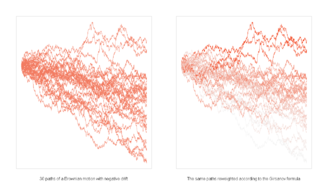
\includegraphics[bb=0 0 320 189]{Girsanov.png}
 % Girsanov.png: 320x189 pixel, 72dpi, 11.29x6.67 cm, bb=0 0 320 189
\end{center}
The graph shows two different measures the one on the right has its measure changed. 
Let $\theta \in \Iloc(Prog)$ (T$\in (0,+\infty) is fixed )$
We need to verify the Novikov condition. Then, under $\Pbb^\theta,$ $t \Rightarrow \hat{W}_t =W_t - \int_0^t \theta_s ds
 $ is a $\Fcal_t-BM$ on $[0,T]$
\end{theorem}
\begin{remark}
 A sequence of Girasnov that the laws W and $\hat{W}$ are equivalent on every interval $[0,T]$ 
Indeed: assume that $\Pbb(W|_{[0,T]} \in A) = 0$\newline
$\Pbb(\hat{W} \in A) = \Ebb^{\theta}(\Ind_{(\hat{W} \in A)}(Z^\theta_T)^{-1})=0,$\newline
since $\hat{W}$ is a B.M. under $\Pbb^\theta$\newline
If $\Pbb(\hat{W} \in A) = \Ebb^\theta(\Ind_{\hat{W} \in A}(Z^\theta_T)^{-1})$ since $(Z^\theta_T)^{-1} >0$ by definition
\newline $\Rightarrow\; \Ind_{(\hat{W} \in A)}=0$ a.e. $d\Pbb^{\theta}$
\newline $\iff \Ind_{(W \in A)} = 0$ a.e. $d \Pbb$
\end{remark}
\begin{proof}[Of Girasnov's theorem]
 We just consider the case ``$\theta_s$ is deterministic''
We know - $\hat{W}_t$ is continuous, $\hat{W}_0 = 0$, $\hat{W}_t$ is $\Fcal_t$-progressive
$(\Rightarrow \Fcal_t - \mathrm{adapted})$
Everything we need to show is that \[\forall 0 \leq t_0 < t_1 < t_2 <\cdots < t_k \leq T \]\[
(\hat{W}_{t_1}-\hat{W}_{t_0}, \cdots , \hat{W}_{t_k}- \hat{W}_{t_k-1}) \sim
\Ncal \left(0,
	\begin{pmatrix}
		t_1 - t_0 & 0 & \cdots & 0 & 0 \\
		0 & t_2 - t_1 & \cdots & 0 & 0 \\
		\vdots & \vdots & \ddots & \vdots & \vdots \\
		0 & 0 & \cdots & t_{n-1} - t_{n-2} & 0 \\
		0 & 0 & \cdots & 0 & t_n - t_{n-1}
	\end{pmatrix}
\right).
\]
Fix $(\lambda_1,\cdots, \lambda_k) \in \Rbb^k$
\newline $\Ebb^{\theta} [\exp{i \sum_{j=1}^{k} \lambda_{j}(\hat{W}_{t_{j}}-\hat{W}_{t_{j-1}}))}]$(\textasteriskcentered)
\newline It is worth pointing out that a Goal of this section is to show that $exp{-\frac{1}{2} \sum_{j=1}^{k}
\lambda^{2}_j(t_j - t_{j-1}}) = \textasteriskcentered$
\newline = $\Ebb^{\theta}[{\exp{i \sum_{j=1}^{k} \lambda_j(W_{{t}_{j}} - W_{{t}_{j-1}} - \int_{{t}_{j-1}}^{t_{j}}]
\theta_{s} ds}}$
= $\Ebb(\exp{i \sum_{j=1}^{k} \lambda_j(W_{t_{j}} - W_{t_{j-1}} - \int_{{t}_{j-1}}^{{t}_{j}}Z^{\theta}_T)}$
\newline = $\Ebb[{\exp{i \sum_{j=1}^{k} \lambda_j(W_{{t}_{j}} - W_{{t}_{j-1}} - \int_{{t}_{j-1}}^{{t}_{j}}\explainup{Z^{\theta}_{t_{k}}}{(\textrm{martingale property under}\; \Pbb)}}} ]$
\newline = \begin{equation}\label{Girasnov}
\Ebb[{\exp{i \sum_{j=1}^{k} \lambda_{j}(W_{t_{j}}-W_{t_{j-1}} - \int^{t_{j}}_{t_{j-1}} \theta_s ds)} 
\exp{\int^{t_{k}}_{0} \theta_s dW_s - \frac{1}{2} \int^{{t}_{k}}_{0} \theta^{2}_s ds}}]\end{equation}
(we can assume without loss of generatlity that $t_0 = 0$)
Now we can write
$\int_0^{t_{k}}\theta_s dW_s$ and $\int^{t_{k}}_{0} \theta^{2}_s ds = \sum_{j=1}^{k}\int^{t_{j}}_{t_{j-1}} \theta^{2}_s ds$
So that 
\newline \ref{Girasnov}= $\Ebb[\exp{\sum_{j=1}^{k}\int_{t_{j-1}^{t_{j}(i\lambda_{j} + \theta_{s})dW_{s} -
\sum_{j=1}^{k}\int^{t_{j}}_{t_{j-1}} i \lambda_{j} \theta_{s} ds - \frac{1}{2}} }}]$
\end{proof}

\end{document}


